\documentclass[
% -- opções da classe memoir --
12pt,				% tamanho da fonte
openright,			% capítulos começam em pág ímpar (insere página vazia caso preciso)
oneside,			% para impressão em verso e anverso. Oposto a oneside
a4paper,			% tamanho do papel. 
% -- opções da classe abntex2 --
%chapter=TITLE,		% títulos de capítulos convertidos em letras maiúsculas
%section=TITLE,		% títulos de seções convertidos em letras maiúsculas
%subsection=TITLE,	% títulos de subseções convertidos em letras maiúsculas
%subsubsection=TITLE,% títulos de subsubseções convertidos em letras maiúsculas
% -- opções do pacote babel --
english, % idioma adicional para hifenização
french, % idioma adicional para hifenização
spanish, % idioma adicional para hifenização
brazil % o último idioma é o principal do documento
]{abntex2}

% --- Pacotes básicos ---
\usepackage{lmodern} % Usa a fonte Latin Modern
\usepackage[T1]{fontenc} % Selecao de codigos de fonte.
\usepackage[utf8]{inputenc} % Codificacao do documento (conversão automática dos acentos)
\usepackage{lastpage} % Usado pela Ficha catalográfica
\usepackage{indentfirst} % Indenta o primeiro parágrafo de cada seção.
\usepackage{color} % Controle das cores
\usepackage{graphicx} % Inclusão de gráficos
\usepackage{microtype} % para melhorias de justificação
\usepackage{pgf,tikz}
\usepackage{mathrsfs}
\usepackage{amsmath}
\usepackage{amssymb}
\usepackage{float}
\usetikzlibrary{patterns,arrows,decorations.pathreplacing}

% ---

% --- Pacotes adicionais, usados apenas no âmbito do Modelo Canônico
% do abnteX2 ---
\usepackage{lipsum} % para geração de dummy text
% ---

% --- Pacotes de citações

\usepackage[alf]{abntex2cite} % Citações padrão ABNT
\usepackage{verbatim} \usepackage[colorinlistoftodos]{todonotes}
\usepackage{soul}
% --- CONFIGURAÇÕES DE PACOTES ---

% ---

% ---

% --- Informações de dados para CAPA e FOLHA DE ROSTO ---
\titulo{Emergência de Distribuições de Preferência no caso Unidimensional: Uma abordagem computacional}
\autor{Marcelo Veloso Maciel} \local{Brasil} \data{2017}
\orientador{André Cavalcanti Rocha Martins}

\instituicao{%
  Universidade de São Paulo -  USP
  \par
  Escola de Artes, Ciências e Humanidades - EACH
  \par
  Mestrado em Modelagem de Sistemas Complexos} \tipotrabalho{Dissertação de Mestrado)}
% O preambulo deve conter o tipo do trabalho, o objetivo, o nome da
% instituição e a área de concentração
\preambulo{\textcolor{red}{ Informações sobre a qualificação }}
% ---


% --- Configurações de aparência do PDF final

% alterando o aspecto da cor azul
\definecolor{blue}{RGB}{41,5,195}

% informações do PDF
\makeatletter \hypersetup{
  % pagebackref=true,
  pdftitle={\@title}, pdfauthor={\@author},
  pdfsubject={\imprimirpreambulo}, pdfcreator={LaTeX with abnTeX2},
  pdfkeywords={abnt}{latex}{abntex}{abntex2}{trabalho acadêmico},
  colorlinks=true, % false: boxed links; true: colored links
  linkcolor=blue, % color of internal links
  citecolor=blue, % color of links to bibliography
  filecolor=magenta, % color of file links
  urlcolor=blue, bookmarksdepth=4 } \makeatother
% ---

% --- Espaçamentos entre linhas e parágrafos ---

% O tamanho do parágrafo é dado por:
\setlength{\parindent}{1.3cm}

% Controle do espaçamento entre um parágrafo e outro:
\setlength{\parskip}{0.2cm} % tente também \onelineskip

% --- compila o indice ---
\makeindex
% ---

% ---- Início do documento ----
\begin{document}
	
	% Seleciona o idioma do documento (conforme pacotes do babel)
	%\selectlanguage{english}
	\selectlanguage{brazil}
	
	% Retira espaço extra obsoleto entre as frases.
	\frenchspacing 
	
	% ----------------------------------------------------------
	% ELEMENTOS PRÉ-TEXTUAIS
	% ----------------------------------------------------------
	% \pretextual
	
	% ---
	% Capa
	% ---
	\imprimircapa
	% ---
	
	% ---
	% Folha de rosto
	% (o * indica que haverá a ficha bibliográfica)
	% ---
	\imprimirfolhaderosto*

%	\begin{agradecimentos}
%\textcolor{red}{lalalallal}
		
   	
%	\end{agradecimentos}
	
%	\begin{epigrafe}
%		\vspace*{\fill}
%		\begin{flushright}
%			\textit{ \textcolor{red}{lalalla}	}
%		\end{flushright}
%	\end{epigrafe}
	
%	\setlength{\absparsep}{18pt} % ajusta o espaçamento dos parágrafos do resumo
%	\begin{resumo}
%		[Resumo]
 %               \textcolor{red}{lalalala}
		
	%	\textbf{Palavras-chave}:lalala
	%\end{resumo}
	
	% resumo em inglês
	%\begin{resumo}[Abstract]
%		\begin{otherlanguage*}{english}
%	 \textcolor{red}{lalalala in english}
			
%			\vspace{\onelineskip}
			
%			\noindent 
%			\textbf{Keywords}: \textcolor{red}{lalalala}
%		\end{otherlanguage*}
%	\end{resumo}
	
	% ---
	% inserir lista de ilustrações
	% ---
	\pdfbookmark[0]{\listfigurename}{lof}
	\listoffigures* 
    
	\cleardoublepage
	% ---
	
	% ---

	
	% ---
	
	% ---
	
% ---
\begin{siglas}
\item[ABM] \textit{Agent-based model(s) or modeling}
  \item[OD] \textit{ Opinion Dynamics}
 
\end{siglas}
% -
	% ---
	% inserir o sumario
	% ---
	\pdfbookmark[0]{\contentsname}{toc}
	\tableofcontents*
	\cleardoublepage
	% ---
	\textual
	
	%-----
	
	
\chapter*[Introdução]{Introdução}
	    \addcontentsline{toc}{chapter}{Introdução}
      Uma característica chave da Democracia é a responsividade do governo às
preferências, crenças e atitudes dos cidadãos
\cite{dahl1989democracy,bartels2003democracy}. Nas democracias modernas isso
ocorre por meio de vários mecanismos de conexão entres os cidadãos e seus
representantes \cite{dahl1989democracy, schumpeter2013capitalism}. As
Democracias estão, desta forma, fundamentadas no nexo entre Opinião Pública e
Governo Representativo. A natureza e origem da Opinião Pública é então central
para a compreensão dos nossos sistemas políticos \cite{berelson1952democratic}.
Como argumentado por \citeonline{downs1999teoria} a distribuição da Opinião
Pública é de alta relevância para a compreensão do nexo democrático na medida em
que orienta o comportamento de políticos e partidos. Seguindo Downs, o
pressuposto central deste trabalho é que não só a Opinião Pública importa, mas,
mais especificamente, o seu formato também. A literatura em ciência política que
busca explicar, por meio de modelos explícitos, o procedimento de surgimento e
dinâmica de padrões de opinião ainda é escassa e desconectada dos trabalhos em
Dinâmicas de Opinião, uma das principais áreas em Simulação Social
\cite{lorenz2017modeling, laver2011party, hauke2017recent}. Há assim espaço para
a contribuição de trabalhos de caráter generativo, isto é, guiados pela seguinte
pergunta: ``Como pode a interação local entre agentes autônomos heterogêneos
gerar a seguinte regularidade?'' \cite{epstein2006generative}.

Pensar em termos generativos nos leva à busca dos microfundamentos das
regularidades de interesse. Todas as interações sociais são ao menos em parte
condicionadas pelas crenças e opiniões dos agentes. É plausível que haja tanto
um fundamento genético-evolucionário para nossas crenças e orientações, quanto
uma fundamentação em mecanismos relacionados a sistemas de herança e
aprendizados sociais \cite{jablonka2014evolution, fowler2008biology,
  fowler2013defense}. Um indivíduo ao tomar uma decisão não baseia-se unicamente
na informação e crença averiguadas individualmente, mas também pode considerar
as crenças de outros agentes conectados a ele socialmente e informacionalmente
\cite{gintis2016individuality}. Em política isso significa que as crenças dos
agentes são uma combinação de sua crença ``idiossincrática'' e da combinação de
mensagens/sinais que recebem dos seus pares e da mídia
\cite{barabas2004deliberation,ryan2011social}. A ``cognição em rede''
\cite{gintis2016individuality} dos agentes e essas duas fontes de informação,
pares e mídia \footnote{O trabalho trata unicamente dos pares como fonte de
  informação. Modelar a influência da mídia é tema para trabalhos futuros.},
fornecem assim os dois mecanismos mínimos para micro-fundamentar abordagens
generativas para a Opinião Pública.

Tendo em vista esses dois mecanismos, este trabalho, tem por \textbf{objetivo
  geral} explorar, por meio de um modelo baseado em agentes de influência
social, a geração de distribuições de preferências \footnote{A diferença entre
  crenças, preferências e opiniões será discutida nos Capítulo 2 e 3.} análogas
a distribuições empíricas. O fazemos por meio da adaptação do modelo de
\citeonline{martins2009bayesian}. Esse modelo em particular é escolhido por
estar no meio do espectro entre modelos complicados e simples demais do ponto de
vista cognitivo, além de sua influência bayesiana ser coerente com o
\textit{framework} do ator racional\footnote{Essas questões são discutidas no
  Capítulo 3.}. As modificações foram as seguintes: primeiramente, seguimos a
recomendação metodológica de \citeonline{macy2015signal} e incluimos ruído na
dinâmica do modelo; segundo, os posicionamentos dos agentes no espectro político
são derivados dos posicionamentos deles em várias questões, o que é mais
consistente com o fato de que alternativas preferidas por agentes em contextos
de massa são derivadas das atitudes deles em diferentes questões; ademais,
adicionamos agentes intransigentes à população, o que é uma variante,
possibilitada pelo modelo de \citeonline{martins2009bayesian}, da verificação do
papel de extremistas\footnote{ Os extremistas são inseridos nos modelos com o
  intuito de investigar quais propriedades de agentes e de suas interações levam
  ao consenso, à populações isoladas ou polarizadas, dado que isso é tema
  constante de debate e reflexão política e um dos problemas de pesquisa
  centrais para a área de Dinâmicas de Opinião, \cite{fiorina2005culture,
    pulick2016, bramson2016disambiguation}.} na dinâmica de opinião
\cite{deffuant2002can, flache2017}. O modelo foi analisado por meio da
combinação de análise de sensibilidade, histogramas e séries temporais de
medidas do sistema e gráficos de dispersão, com o intuito de verificar em que
medida essas modificações levam a mudanças de comportamento em contraste ao
modelo original e quais os efeitos dos atributos dos agentes e parâmetros do
modelo sobre a opinião populacional, mais precisamente sobre a dispersão e
cobertura das opiniões\footnote{Ambas medidas de
  polarização discutidas no Capítulo 4.}.

Além desta Introdução, o trabalho é estruturado da seguinte forma: no Capítulo 2
caracterizamos e justificamos o problema do trabalho. Para tal fazemos uma
apresentação do modelo do ator racional e sua aplicação para modelar opinião
pública; no Capítulo 3 fazemos uma revisão de literatura dos modelos canônicos
da área de dinâmicas de opinião e fazemos uma discussão sobre nossa abordagem;
no Capítulo 4 apresentamos o modelo, metodologia de análise e resultados;  por
fim nas Considerações Finais apresentamos limitações do trabalho.









\chapter{Teoria Política Formal e Distribuição de Preferências}
Como discutido na introdução, o nexo entre cidadãos e governo é a base dos
sistemas democráticos. Dada a importância desse nexo, não é surpresa que na
Ciência Política exista uma grande gama de trabalhos e abordagens que busquem
descrever, explicar e prevê-lo. A caracterização e
justificativa para nosso problema de pesquisa parte de um diálogo com a Teoria
Política Formal, a ser definida e discutida em seguida.

\section{Fundamentos da Teoria Política Formal}

Vamos definir Teoria Política Formal como: conjunto de modelos e hipóteses
teóricas explicitamente definidos que buscam representar atividades e
comportamentos relacionados à ação e escolha coletiva.

Com essa definição estamos conjugando três definições: a de Teoria, a de
Política e a de Formal. O conceito de política, e em certa medida o de teoria,
pode ser considerado como ``essencialmente contestado'', isto é, é um conceito
cuja grande importância normativa faz com que haja uma disputa em relação à sua
definição e uso\cite{collier2006essentially}. Existe assim ampla literatura
lidando com a melhor definição do que é política. Vamos usar a definição
dada por Joe Oppenheimer, para o qual  a ``política consiste
no comportamento realizado com o objetivo de tomar decisões centralizadas para
um grupo, ou para assegurar o interesse de membros desse grupo'' \cite[p.
I]{oppenheimer2012principles}\footnote{Essa definição é equivalente a dada por
  \citeonline{barber2003strong}. Para uma discussão mais aprofundada sobre o
  tema ver: \citeonline{warren1999political}.}.

Quanto a definição de teorias estamos seguindo perspectivas pós-positivistas de
ciência, particularmente a Visão Semântico-Pragmática de
\citeonline{clarke2012model} em que teorias são conjuntos de modelos, pensados
como representações de sistemas concretos, e hipóteses teóricas - a delimitação
da similaridade dos modelos com determinados sistemas alvo\footnote{Para uma
  discussão sobre as diferentes visões sobre o que são teorias e modelos ver
  \citeonline{sep-structure-scientific-theories}.}.

Por fim, entendemos que os modelos são formais na medida em que construídos por
meio de algum sistema formal \cite{wong2015formal}. Em Teoria Política Formal
isso significa que tendem a ser construídos usando o intermédio da lógica formal,
matemática ou computação \cite{morton1999methods}. Nosso foco na literatura em
teoria política formal é justificado pelo fato dela ser um corpo teórico
construído por meio de modelos \textit{explícitos} \cite{epstein2008model}, de
forma que a seguinte relação fique clara:

\begin{figure}[H]
  \centering 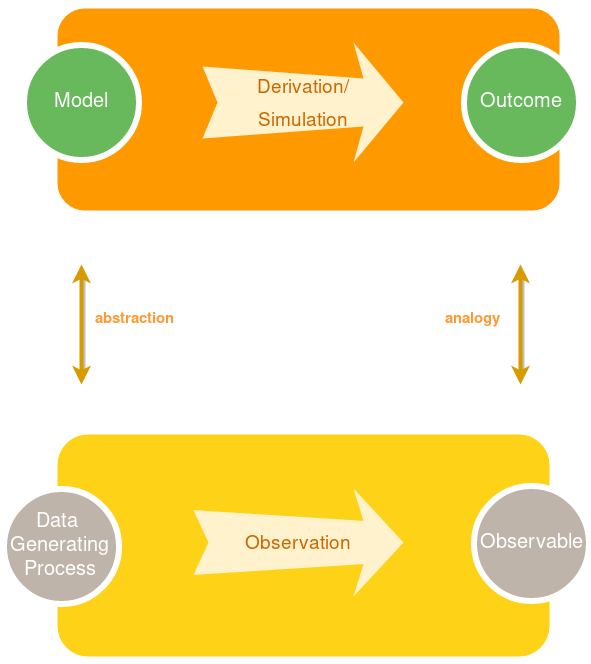
\includegraphics[scale = 0.5]{ims/ms.png}
  \caption{Relação entre Modelos e Sistemas Alvo.}
  Fonte: Adaptado de \citeonline{downey2012think}
\end{figure}

O estudo formal da ação e escolha coletiva teve como período de fundação moderno
o período entre \citeonline{black1948rationale} (marco no estudo da escolha coletiva)
e \citeonline{olson1965logic} (marco para os estudos da ação coletiva), embora
\textit{insights} típicos da literatura, como paradoxos da agregação ou o
problema do caroneiro, tenham sido discutidos anteriormente por pensadores como
Plínio, o Jovem (64-114 d.C.); Ramon Lull (1232-1315); David Hume; e John Stuart
Mill \cite{mclean2015strange, sep-free-rider, ordeshook1990emerging}. 


Embora não seja a única forma de se modelar formalmente fenômenos políticos,
modelos de escolha racional são em larga medida os mais comuns
\cite{austen1998social}. De uma forma geral, os modelos da Teoria da Escolha
Racional, em política, buscam representar fenômenos segundo alguma variante da
seguinte equação, a Equação de Plott \cite{munger2015choosing,
  ostrom1986agenda}\footnote{Essa ``equação'' é conceitual. \(\oplus\) é usado como
  um operador abstrato não especificado \cite{ostrom1986agenda}. }:
\begin{figure}[H]
\begin{align*}
  \text{Preferences} \oplus \text{Beliefs}  \oplus  \text{Physical Possibilities} \oplus \text{Institutions} = \text{Outcomes}
\end{align*}
\end{figure}
O conjunto de modelos conhecidos como ``Teoria da Escolha Racional'' podem ser
dividido em duas variantes: \textit{thin} ou \textit{thick}
\cite{hechter1997sociological, green1996pathologies}. Ambos os tipos de modelos
são construídos com base nos pressupostos mínimos de um modelo de ator racional:
preferências racionais e racionalidade bayesiana \cite{gintis2016individuality}.
A diferença entre eles é que os modelos \textit{thin} não fazem pressupostos
substantivos sobre os valores e objetivos dos agentes. Neles os teóricos buscam
modelar a combinação entre agentes e instituições da maneira mais geral
possível. Já modelos \textit{thick} adicionam um conjunto de pressupostos extras
sobre objetivos, valores, incerteza, com o objetivo de representar fenômenos
particulares como o comparecimento às urnas, a competição partidária, a escolha
de candidatos pelo eleitorado, independência burocrática, o efeito fiscal de
constituições, dentre outros \cite{bendor2011behavioral}.

Todo modelo formal da escolha racional em política envolve os seguintes
elementos primitivos: o conjunto $N$ de agentes, o conjunto \(X\) de
alternativas possíveis, e para cada agente em \(N\) uma descrição de suas
preferências em relação às alternativas em \(X\) \cite[p.
263]{austen1998social}.

A preferência é uma relação de comparação de valor, onde dois conceitos são
fundamentais: o de melhor (preferência estrita), denotado por \(\succ\) e o de igual
em valor (indiferença), denotado por \(\sim\). As seguintes propriedades definem a
noção lógica de relação de preferência \cite{sep-preferences}:

\begin{enumerate}
\item \textit{Assimetria da preferência}: \( x \succ y \to \neg (y \succ x )\); 
\item \textit{Simetria de indiferença}: \(x \sim y \to  y \sim x\); 
\item \textit{Reflexividade da indiferença }: \(x \sim x\); 
\item \textit{Incompatibilidade entre preferência e indiferença}: \(x \succ y \to \neg ( x
  \sim y)\).
\end{enumerate}

A relação de preferência fraca \( \succeq \)pode ser definida da seguinte forma:

\begin{align*}
  \text{x} \succeq y \leftrightarrow x \succ y \lor x \sim y
\end{align*}

A aplicação dessa definição de preferência no modelo do ator racional pressupõe
que ela seja uma relação binária no conjunto de alternativas \(X\), com as
seguintes propriedades, para todo \(x,y,z\) $\in$ \(X\), e para todo conjunto
\(Z\) $\subset$ \(X\) \cite{gintis2016individuality,
  binmore2008rational}:



\begin{enumerate}
\item \textit{Completude}: \(\{ x \succeq y | \vspace{0.4cm} X \}\) ou \(\{ y \succeq x |
  \vspace{0.4cm} X \}\);
\item \textit{Transitividade}: \( \{x \succeq y | \vspace{0.4cm} X\} \) e \(\{y \succeq z |
  \vspace{0.4cm} X \}\) tem por implicação \(\{x \succeq z | \vspace{0.4cm} X\}\);
\item \textit{Independência das alternativas irrelevantes}: para \(x,z \in Z\),
  \(\{x \succeq y | \vspace{0.4cm} Z \}\) se e somente se \(\{x \succeq y | \vspace{0.4cm}
  X\}\).
\end{enumerate}

Um pressuposto adicional é que existe um \(x \in X\) tal que para todo \(y \in X\),
\(x \succeq y\), e que num ambiente sem restrição os atores escolhem essa alternativa
\cite{gintis2009bounds}. Esses pressupostos constituem o primeiro princípio do
modelo do ator racional: os agentes possuem \textit{preferências consistentes ou
racionais}, o que significa que são completas, transitivas e independentes de
alternativas irrelevantes.

Uma conveniência analítica é representar relações de preferência por meio de
funções de utilidade, que são funções que atribuem um número real para cada
elemento do conjunto de alternativas \cite{sep-preferences}. A relação \( \succeq\) é
representada pela função \(u\): \(X \longrightarrow \mathbb{R}\) se e somente se:

\begin{align*}
  u(x) \geq u(y)
  \text{ se e somente se }
  x \succeq y
\end{align*}

Por meio dessa representação, a alternativa preferida, ou ótima, para um ator $i
\in N$ é dada por \cite{binmore2008rational}:
\[\max_{\substack{x \in  X}}
  u_i(x)
\]

Importante notar que funções de utilidade são um dispositivo matemático. Modelar
agentes por meio de funções de utilidade 
não implica que eles sejam  egoístas, instrumentais, utilitários,
hedonistas, ou que estejam ``tentando maximizar sua utilidade''
\cite{gaus2007philosophy}.

O segundo princípio dos modelos de ator racional é a \textit{racionalidade
  bayesiana} \cite{gintis2016individuality}. Quando as alternativas são
probabilísticas primeiro pressupomos que os agentes tem um \textit{modelo do
  mundo}\cite{acemoglu2011opinion}: os agentes vão ter uma crença, representada
por meio de uma função de distribuição de probabilidade\footnote{O modelo da
  escolha racional então pressupõe que as crenças dos agentes são coerentes ou
  consistentes, o que equivale a dizer que estão em conformidade com os axiomas
  da probabilidade \cite{jackman2009bayesian}.}, a qual vai atribuir uma
probabilidade \(p\) para cada evento em \(X\). A partir disso pressupõe-se que
agentes vão ter uma relação de preferência sobre
\textit{apostas}\cite{jehle2001advanced}, onde o conjunto de apostas
\(\mathcal{G}\) em \(X = \{ x_1, \ldots, x_n \}\) é dado por:

\begin{align*}
  \mathcal{G} \equiv \big{\{}  (p_1 \circ x_1, \ldots, p_n \circ x_n  ) | p_i \geq 0, \sum_{i = 1 }^n p_i = 1  \big{\}}  
\end{align*}

Sendo assim, quando as alternativas são probabilísticas o modelo do agente
racional pressupõe que os agentes vão ter uma função de utilidade esperada \(u:
\mathcal{G} \to \mathbb{R} \):

\begin{align*}
  u(\mathcal{G}) = \sum_{i =1}^n p_i u(x_i)
\end{align*}

O último elemento do princípio da \textit{racionalidade bayesiana} é a
\textit{atualização bayesiana}\cite[p.104]{gintis2016individuality}: os agentes
atualizam suas crenças segundo a Regra de Bayes.

Sendo assim, os modelos de escolha racional na sua versão mais básica pressupõem
agentes com preferências consistentes, o que implica que sejam transitivas,
completas e independente de alternativas irrelevantes. Caso o contexto de
decisão seja incerto também pressupõem que os agentes tem uma crença em
conformidade com os axiomas da probabilidade, agem de acordo com princípio da
utilidade esperada e atualizam suas crenças de acordo com o Teorema de Bayes.



\section{Teoria Política Espacial}
 













\chapter{chap2}


 Nesse capítulo fazemos uma revisão bibliográfica da área de Dinâmicas de
Opinião (OD). Definimos a área, o
que são modelos baseados em agente e quais os constituintes típicos de um modelo
de OD. Depois apresentamos modelos que inspiraram uma gama de modificações e
extensões. Na seção seguinte discutimos algumas questões teóricas referentes à
atualização da opinião dos agentes e concluímos o capítulo com uma discussão de
nossa abordagem.


\section{Definição da Área}

OD é uma área que pode ser definida a partir de 3 elementos. Primeiramente,
sistemas alvo, fenômenos de interesse, em comum, delimitados pela pergunta
central: quais elementos determinam se um grupo de agentes chega ao consenso
sobre algo, ou ao invés disso persistem em discórdia?
\cite{castellano2012social}\footnote{Essa pode ser pensada como a pergunta
  \textit{fundacional} da área \cite{flache2017}.}. Segundo, um conjunto de
modelos que partilham elementos constitutivos, particularmente fazendo uso da
técnica da Modelagem Baseada em Agentes (ABM), e em, alguma medida, de
\textit{insights} e técnicas da Física Estatística \cite{galam1990social}.
Terceiro, uma comunidade de pesquisadores que partilham do interesse no objeto,
fazem uso de referenciais e técnicas compartilhadas e se reconhecem como membros
dessa comunidade.

Na área há a aceitação de um significado amplo e abstrato de opinião como uma
característica de um agente que pode ser mudada com pouco custo
\cite[p.312]{castellano2012social}. Isso permite com que os pesquisadores visem
sistemas alvos tais como voto, ciência, cultura, difusão de tarifas, dentre
outros
\cite{kowalska2013going,martins2015thou,axelrod1997dissemination,galam1990social}.
Essa gama de aplicações está relacionada com a base disciplinar dos
pesquisadores, envolvendo pessoas de áreas como Física, Sociologia, Ciência
Política, Economia, Psicologia Social, dentre outras, o que nos permite
considerar a área como um subgrupo da Sociofísica
\cite{galam1982sociophysics,galam2012sociophysics}.


\section{Modelagem Baseada em Agentes e Dinâmicas de Opinião}

Modelos Baseados em Agentes podem ser definidos como modelos que envolvem
agentes discretos, onde agentes, seus atributos, e possivelmente um ambiente são
definidos algoritmicamente \cite{sayama2015introduction} \footnote{ ABMs
  costumam ser implementados como simulações num computador, embora existam
  modelos baseados em agentes que historicamente não tenham sido diretamente em
  computadores, como os modelos de Schelling e de Sakoda
  \cite{hegselmann2017thomas}.}. Num ABM existem três noções primitivas: os
\textit{atributos}, os \textit{estados} e as \textit{configurações}
\cite{de2014agent}. Os atributos dos agentes são o conjunto de propriedades
que cada cada agente \(i\) tem. Os estados dos agentes são os valores de seus
atributos num determinado tempo \(t\). Já as configurações são as coleções de
todos os estados dos agentes num modelo.

ABM é uma técnica flexível: podemos construir modelos metafóricos com
objetivo de auxiliar o desenvolvimento de intuição segundo a elucidação de
princípios; ou de alta-fidelidade, com dezenas de atributos e um
ambiente incluindo casas, escolas, sistemas de transporte, dentre outros, com o
objetivo avaliar contrafactuais próximos a determinados casos concretos
\cite{de2014agent, epstein2006generative}.


Segundo \citeonline[p.430-1]{sayama2015introduction}, ABMs têm as seguintes
propriedades típicas:
\begin{itemize}
\item agentes podem ter estados internos;
\item agentes podem ser espacialmente localizados;
\item agentes podem perceber e interagir com o ambiente;
\item agentes podem interagir segundo regras pré-definidas;
\item agentes podem ser capazes de aprender e adaptar-se;
\item agentes podem interagir com outros agentes;
\item AMBs muitas vezes não tem supervisores/controladores centrais;
  \item ABMs podem produzir comportamentos coletivos não triviais.
  \end{itemize}

  Tendo em vista essas propriedades, ABMs são particularmente úteis para o
  estudo de sistemas complexos \cite{wilensky2015introduction}, dada: sua
  capacidade de incluir redes e espaço; seu potencial de ligar múltiplos
  domínios e de incluir uma maior heterogeneidade de agentes; além de seu foco
  na robustez de resultados \cite{de2014agent,wilensky2015introduction}. ABMs
  são assim capazes de conectar como propriedades macro surgem a partir das
  regras de interação e atributos dados a unidades discretas, os agentes
  \cite{north2007managing}. Não por acaso, ABMs são amplamente usados em OD
  \cite{castellano2012social,flache2017}.

  Essas propriedades são ditas emergentes na medida em que caracterizam o
  sistema e não seus componentes. Isto é, propriedades emergentes são aquelas
  que resultam da interação entre as partes do sistema, mas que não seriam a
  priori dedutíveis unicamente das propriedades delas. O conceito, modernamente,
  é relativo tanto ao quadro conceitual quanto às expectativas dos pesquisadores
  sobre quais propriedades sistêmicas poderíamos deduzir a partir das
  propriedades das partes \cite{epstein2006generative}. Em sua forma mais
  simples propriedades emergentes condicionam indiretamente o comportamento dos
  agentes. Se os agentes tiverem consciência dessa propriedade sistêmica temos,
  contudo, um \textit{feedback} direto, ao invés de indireto, entre agentes e
  propriedades sistêmicas, o que \citeonline{squazzoni2008micro} chama de
  emergência de segunda ordem. No nosso trabalho lidamos somente com
  \textit{feedbacks} indiretos, ou emergência de primeira ordem.\todo[color =
  yellow!10]{talvez falar mais disso...}

  Que elementos constituem os modelos de OD ? Podemos delimitar um modelo de
  dinâmicas de opinião da seguinte forma: agentes conectados possuem opiniões
  como variáveis e interagem segundo regras que explicam a mudança ou manutenção
  das opiniões individuais sob efeito da interação com outros agentes ou outras
  fontes (como a mídia) \cite{sirbu2017opinion}. Os agentes num modelo em OD têm
  então: uma \textit{opinião}; uma \textit{estrutura de interação}; e uma
  \textit{regra de atualização} de sua opinião.


  A opinião dos agentes pode ser representada como uma variável ou conjunto de
  variáveis, que por sua vez podem ser discretas ou contínuas. Já a estrutura de
  interação consiste no conjunto de agentes cujas ações e propriedades podem
  afetar a opinião de um agente \(i\) \cite{page2008uncertainty}.

  Podemos dividir a estrutura de interação numa \textit{topologia} de interação e
  numa \textit{regra de interação}. A topologia de interação define quais
  agentes estão conectados com \(i\), e podem, potencialmente, afetá-lo. A regra
  de interação define como \(i\) interage com os agentes desse conjunto(seus
  ``vizinhos''). Em OD as regras de interação definem qual a
  relação que o agente \(i\) tem com seus vizinhos: se interage com um vizinho
  por vez, uma interação em díade, ou com algum subconjunto de seus vizinhos,
  uma interação em grupo. Por fim, a regra de atualização define sob qual regra
  a opinião do agente \(i\) muda do tempo \(t\) para o tempo \(t+1\). 

  

  \section{Modelos Canônicos}

  Adaptações do Modelo de Ising são os modelos mais fundamentais na área. O
  modelo de Ising é um modelo paradigmático da Mecânica Estatística, usado para
  representar o processo de magnetização de materiais\footnote{O modelo de Ising
    é um modelo paradigmático de sistemas com muitas partes interagindo levando
    à uma transição de fase, a uma mudança de comportamento qualitativo do
    sistema. Sendo assim, é aplicado em vários contextos além da sua concepção
    original, como mercados financeiros, sistemas ecológicos, e dinâmicas de
    opinião \cite{sole2011phase}}. Nestes, variáveis discretas, \textit{spins},
  com valores $s = \pm 1$, estão localizadas num grafo e têm uma tendência a
  alinhar-se com seus vizinhos: se a maioria tem \(s = + 1 \) o spin muda seu
  valor para \(+1\); se a maioria tem \(s = -1 \) o spin muda seu valor para
  \(-1\); se houver empate o spin muda seu valor com probabilidade
  \(\frac{1}{2}\) \cite{castellano2012social,sole2011phase}. A reinterpretação
  para o contexto de OD é o seguinte: o spin é um agente; sua opinião pode ter
  os valores \(+1\) ou \(-1\); um agente interage com todos seus vizinhos por
  passo de tempo; ele assume a opinião da maioria deles.

  Um modelo parecido com o anterior é o ``Voter'' \cite{holley1975ergodic}. Neste
  cada agente tem uma opinião binária \(\pm\) 1 ; e a cada passo um agente é
  selecionado aleatoriamente e assume a opinião de algum de seus vizinhos.
  Difere do modelo anterior, portanto, na regra de interação (díade ao invés do
  grupo inteiro) e de atualização (assume o valor do vizinho ao invés da maioria
  deles).


  Já no modelo da Regra de Maioria a interação é : a cada
  unidade de tempo um grupo
  de tamanho \textit{r} é selecionado aleatoriamente e todos os agentes mudam
  sua opinião para a opinião da maioria do grupo
  \cite{galam1990social,galam2012sociophysics}. O tamanho \textit{r} pode ser
  fixo ou ser tirado de alguma distribuição a cada passo. Se \textit{r} for par
  podem ocorrer empates nos grupos, de forma que ou o grupo escolhe uma das
  opiniões com probabilidade \(\frac{1}{2}\), ou introduz-se um viés, e toda vez
  que houver empate o grupo muda para uma das opiniões
  \cite{galam2012sociophysics, galam1986majority}.

  O Modelo Sznajd também é bastante discutido na literatura
  \cite{sznajd2000opinion, sirbu2017opinion,castellano2012social}. Neste cada
  agente têm exatamente dois vizinhos, em uma grade unidimensional. A cada passo
  um par $ij$ de vizinhos é selecionado e se sua opinião for igual os outros
  vizinhos de \(i\) e \(j\) mudam a opinião para a opinião de convergência. Se
  eles discordarem, \(i\) adota a opinião do outro vizinho, e \(j\) faz o mesmo.

  Todos os modelos até agora representaram opiniões como uma variável que pode
  tomar valores binários. Além disso a regra de atualização dos modelos
  pressupõe uma interação assimilativa: indivíduos conectados por meio de uma
  relação estrutural influenciam uns aos outros em direção à diminuição da
  diferença de suas opiniões \cite{flache2017}. O modelo de
  \citeonline{axelrod1997dissemination} difere em ambos os aspectos. Cada agente
  tem por opinião um vetor $F$ de componentes $(\sigma_1 , \ldots, \sigma_f)$
  \cite{klemm2003role}. Esses $\sigma_i$ podem tomar valores inteiros de 0 a 9. Os
  componentes são as características culturais dos agentes e seus possíveis
  valores são seus traços culturais \cite{gomes2014}. O modelo considera
  interação entre pares de vizinhos, os quais interagem com uma probabilidade
  proporcional ao número de traços que têm igual. Isso significa que se \(i\)
  tem uma opinião igual a 82330 e seu vizinho \(j\) tem uma opinião 67730 eles
  têm \(40 \%\) de interagirem. Se eles interagirem, \(i\) troca um dos traços
  em que difere \(por\) j um dos traços de \(j\)\cite{axelrod1997dissemination}.
  Nesse modelo pessoas similares têm uma probabilidade maior de se interagirem
  do que pessoas distintas, mas uma vez que a interação ocorre elas ficam mais
  parecidas. Sendo assim, o modelo de Axelrod pode ser considerado um modelo de
  assimilação enviesada: só indivíduos suficientemente similares podem
  influenciar uns aos outros na redução de suas diferenças\footnote{Um terceiro
    tipo de modelo elencado por \citeonline{flache2017}, além dos modelos de
    influência social assimilativa e modelos com influência enviesada, são os
    modelos de influência repulsiva: quando agentes são muito distintos em
    opinião a interação pode levá-los a um aumento dessa diferença, isto é,
    tornam-se mais distantes.} \cite{flache2017}.


  Um outro modelo de assimilação enviesada é o Modelo de Deffuant-Weisbuch
  \cite{deffuant2000mixing}. Nele cada agente \(i\) tem opinião inicial \( o_i \in
  [0,1]\). Dois agentes são escolhidos aleatoriamente, e \(i\) é influenciado
  por \(j\) se \(| o_i - o_j| < \epsilon\). Se isso ocorrer suas opiniões se aproximam
  de acordo com um parâmetro $0 < \mu< \leq 0.5$, de forma que: $o_{i,t+1} = o_{it} +
  \mu(o_{jt} - o_{it})$. Esse modelo é particularmente relevante para o presente
  trabalho, por duas razões: a opinião é contínua, assim como a representação
  das ``utilidades'' dos agentes em Teoria Política Espacial \footnote{Na
    verdade, ligar a literatura de OD com funções de utilidade em economia e com
    a noção geométrica de política é a justificativa dada por
    \citeonline{deffuant2000mixing} para considerar opiniões como contínuas.}; e
  \(\epsilon\) pode ser interpretado como parte da regra de atualização, o que faz
  modelo os agentes tenham viés de confirmação.

Quando \(\epsilon\) é interpretado como parte da regra de interação temos o princípio
da homofilia: padrões estruturais de interação social levam pessoas a ter maior
probabilidade de interagirem com pessoas similares a elas
\cite{mcpherson2001birds}. Quando \(\epsilon\) é interpretado como parte da regra de
atualização temos o fenômeno do \textit{viés de confirmação}: a tendência das
pessoas de dar maior peso a informações que confirmem suas crenças anteriores
\cite{nickerson1998confirmation}.

\citeonline{huckfeldt2005patterns} argumenta que indivíduos escolhem redes de
discussão com razões distintas às políticas (como interesses profissionais e
hobbies) e acabam interagindo com indivíduos cujas filiações partidárias
distintas. Desta forma, o papel da homofilia em política é atenuado. Já o
\textit{vies partidário} dos cidadãos, o viés de confirmação no tocante a
questões políticas , é um resultado estabelecido na literatura em opinião
pública e psicologia política, e imprescindível para a modelagem generativa de
opinião pública \cite{bartels2002beyond, flynn2017nature,
  lodge2013rationalizing}.


\section{Regra de Atualização e Processamento de Informação}


Como lembra Dirk Helbing, não existe uma única forma de modelar agentes
interagindo em sistemas sociais complexos \cite{helbing2010pluralistic}. Os
modelos clássicos em OD têm uma abordagem que Helbing chama de
\textit{fisicalista}: abstraem as interações sociais ao ponto delas poderem ser
estudadas como um modelo de ``partículas''. Em OD essa abordagem é refletida na
forma como se modela a regra de atualização: abstrai-se o processamento de
informação, a cognição dos agentes. Isso, como frisa Helbing, não é uma falha
dos modelos. Paul Ormerod defende que o \textit{null model} em sistemas sociais
complexos deveria ser o de um \textit{zero intelligence actor}, pois a
complexidade dos sistemas nos permitiria modelar os agentes ``como se fossem''
átomos \cite{ormerod2008can, bentley2012agents}.

Não obstante, um conjunto de trabalhos em OD tem buscado abrir a ``caixa-preta''
da cognição dos agentes e tratam a atualização de opinião como resultado de um
processamento de informação explicitamente modelado \cite{flache2017,
  jager2017}. O modelo Polias de \citeonline{brousmiche2016beliefs}, o modelo
Innomind de \citeonline{schroder2017modeling} e o modelo Lodge-Taber
\cite{kim2010computational,kim2011model} de processamento dual e raciocínio
motivado são exemplos dessa tendência.

Se pensarmos num espectro possível de abordagens para a cognição dos agentes,
ilustrado na Figura \ref{fig4} , esses modelos estão posicionados no extremo oposto aos
modelos fisicalistas. Enquanto os modelos fisicalistas abstraem totalmente o que
se passa na cabeça dos agentes os modelos (neuro)cognitivos buscam representar a
arquitetura cognitiva que alicerça as atitudes e crenças
deles \cite{kim2010computational}.

\begin{figure}[H]
  \centering
  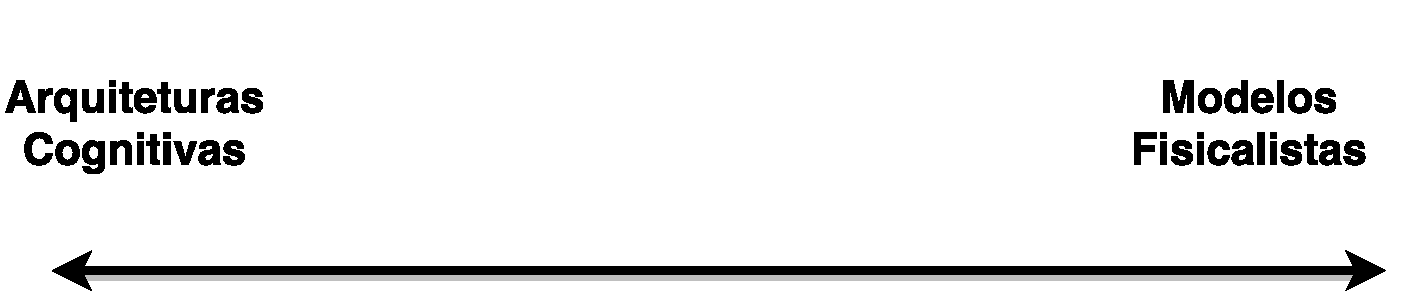
\includegraphics[width = \textwidth, height = 3cm]{ims/line.pdf}
  \caption{Espectro de abordagens no tocante à cognição dos agentes}
  \fonte{O autor.}
  \label{fig4}
\end{figure}

Modelos cognitivamente ``densos'' permitem que analisemos como processos de
influência social estão micro-fundamentados em processos mentais subjacentes, e
são um fronte dentre os trabalhos que buscam aumentar o realismo das simulações
sociais \cite{jager2017,epstein2014agent_zero, conte2013minding}. Contudo, como
ressalta Jonathan Bendor, na medida em que a Ciência Política busca modelar
macrofenômenos ela ``deve ser mais implacável em relação aos micropressupostos
do que microcampos relacionados (como ciência cognitiva)''
\cite[p.45]{bendor2010bounded}. Quanto mais complicados nossos modelos menor
controle temos sobre qual o elemento responsável pelo seus resultados, e mais
dados precisamos para a sua calibração e validação \cite{de2005computational}.
Como argumentado por \citeonline{zaller1992nature}, a estratégia metodológica
para modelar a opinião pública, um fenômeno social de larga escala, envolve
incorporar no modelo somente os aspectos do processamento de informação que têm
relevância para a compreensão das dinâmicas do fenômeno, ao invés de buscar
desenvolver modelos que aproximam o mais próximo o possível os detalhes da mente
humana\footnote{No contexto da análise institucional um argumento equivalente é
  feito por \citeonline{ostrom1990governing}.}.


\citeonline{martins2012bayesian} apresenta um \textit{framework} para modelar
Dinâmicas de Opinião que é cognitivamente mais
``denso'' que os modelos fisicalistas, mas sem buscar modelar as bases
neurocognitivas de processamento de informação. O \textit{framework} está
fundamentado no uso da inferência bayesiana como base da regra de atualização
dos agentes. Embora seja bem documentado que as pessoas não seguem fielmente o
princípio da racionalidade bayesiana, apresentado no primeiro capítulo, um
conjunto de trabalhos em psicologia e ciência cognitiva vêm, nos últimos anos,
defendendo a possibilidade de que sejamos ``bayesianos
imperfeitos''\cite{griffiths2006optimal,fujikawa2007perfect,baker2017rational,
  gintis2016individuality}. Usar um framework bayesiano é, desta forma, uma
aproximação e permite a construção de modelos de dinâmicas de opinião de uma
forma fundamentada num princípio comum, algo particularmente relevante numa área
em que há a proliferação de modelos ad-hoc \cite{flache2017,jager2017}.

 \citeonline[p.214]{martins2012bayesian} oferece o seguinte passo a passo
para a construção de um modelo de dinâmicas de opinião com base num
\textit{framework} bayesiano:

\begin{enumerate}
\item Identificar uma questão sob debate e chamá-la de $x$. \(x\) pode ser
  discreto ou contínuo.
\item cada agente \(i\) tem uma opinião subjetiva sobre $x$ e essa opinião é
  representada pela distribuição de probabilidade $f_i(x)$ .
\item Ocorre comunicação : a comunicação é a declaração de um valor
  $ A_j$ pelo agente $j$ de tal forma que $A_j[f]$ é um funcional de
  $f_j(x)$.
\item Os agentes tem que ter em sua mente  uma relação entre o
  verdadeiro valor entre $x$ e o valor declarado $A_j$. Isso é dado
  pela distribuição de probabilidade $P(A_j|x)$.
\item Dado o prior $f_i(x)$ a opinião posterior $f_i(x|A_j)$ é dada
  por $A_i[f_i(x|A_j)]$ que é a nova opinião de $i$ .
\end{enumerate}





A aplicação desse \textit{framework} no caso de opiniões contínuas incorpora o
mecanismo de viés de confirmação presente no modelo  Deffuant-Weisbuch,
recupera seus resultados qualitativos, e ainda tem resultados adicionais
\cite{martins2009bayesian}. Dado que o modelo representa a atualização de uma
variável contínua, incorpora viés de confirmação e fundamenta a regra de
atualização num framework bayesiano de processamento de informação ele será a base
do nosso trabalho. 

Nele os agentes interagem num grafo completo e a regra de interação é uma díade
interagindo a cada passo de tempo. A opinião inicial dos agentes é dada por uma
probabilidade subjetiva:


\begin{align}
f_i(\theta) = \frac{1}{\sqrt{2 \pi} \sigma_i} e^{-
  \frac{(\theta - o_i )^2}{2 \sigma_i}}
  \end{align}

  Onde \(o_i = E_i[\theta] \), de forma que \(E_i\) é o valor esperado que o agente
  associa a \(\theta\). Para incluir viés de confirmação na regra de atualização,
  \citeonline{martins2009bayesian} introduz uma probabilidade \(p\) que o outro
  agente saiba algo sobre $\theta$ isto é, que tenha uma opinião plausível e que vale
  a pena ser levada em conta ; e vai ter uma chance \(1 - p\) que o outro agente
  não tenha informação sobre $\theta$ de forma que a verossimilhança de $j$ estar
  correto é dado por $ f(o_j|\theta) = p N(\theta,\sigma_j^2) + (1-p)U(0,1)$.

  Temos então que a distribuição da nova opinião é dada por uma mistura de duas
  normais com médias diferentes, que é proporcional à  multiplicação da
  verossimilhança e a distribuição a priori normal de $i$:
  
  \begin{align}
    f(\theta | o_j)
    \propto 
    p
    e^
    {-(\frac{1}{2\sigma_i^2})
    [(\theta - o_i)^2
    +
    (o_j - \theta )^2
    ]}
    +
    (1-p)
    e^{-\frac{(o_i - o_j)^2}{(2 \sigma_i^2)}}
  \end{align}

 Se calcularmos o $E_i(\theta)$ da expressão anterior temos a nova opinião:
  \begin{align}
    o_i(t+1)
    =
    p
    \frac{o_i(t) + o_j(t)}{2}
    +
    (1-p^*)o_i(t)
  \end{align}

  Onde:
  \begin{align}
    p^*
    =
    \frac{
      p \frac{1}{\sqrt{2 \pi} \sigma_i}
      e^{(- \frac{o_i (t) - o_j (t))^2}{2 \sigma_i^2})}
    }{
      p
      \frac{1}{\sqrt{2 \pi} \sigma_i}
    e^{(- \frac{o_i (t) - o_j (t))^2}{2 \sigma_i^2})}
    +
    (1 - p)
    }
  \end{align}

  Importante notar que embora o modelo use a Regra de Bayes para derivar como o
  agente atualiza sua opinião nele o agente não é perfeitamente racional. A
  regra de bayes foi usada para criar uma regra de atualização plausível, mas a
  verossimilhança de um agente perfeitamente racional envolveria considerar
  toda a informação possivelmente relevante
  , por exemplo, se \(j\) tem um interesse estratégico em declarar um
  determinado \(o_j\) ou como \(o_j\) é resultado da interação de j com outros
  agentes. Ademais, suponha que \(i\) e \(j\) interagem num tempo \(t_a\) e
  depois num tempo \(t_b\). Um agente perfeitamente racional corrigiria pela
  repetição da interação \cite{acemoglu2011opinion}, já no modelo de
  \citeonline{martins2009bayesian} o agente age segundo a heurística dada pela
  Equação 2.4. Nele, portanto, os agentes são ``imperfeitamente'' bayesianos.
  Com essa regra de atualização o modelo já recupera os resultados dos modelos
  de confiança limitada. Contudo, também é possível considerar o caso em que a
  incerteza dos agentes é atualizada:

      \begin{align}
    \sigma_i^2(t+1)
    =
    \sigma_i^2(t)
    (1 - \frac{p^*}{2})
    +
    p^*
    (1-p^*)
    (\frac{o_i(t)-o_j(t)}{2})^2
      \end{align}

      Como demonstra \citeonline{martins2009bayesian} essa equação faz com que
      os agentes fiquem mais certos de suas opiniões. Isso é relevante do ponto
      de vista da modelagem generativa de opinião pública.
      \citeonline{kuklinski2000misinformation} encontram que um grande
      percentual,em média \( 60 \%\), dos respondentes em um
      \textit{survey} por telefone sobre questões factuais da agenda política
      americana da época são confiantes em suas crenças. Ademais, encontram uma
      correlação entre confiança e partidarismo. É interessante, portanto,
      incorporar não só a dinâmica da opinião dos agentes, mas também o papel da
      incerteza quanto as crenças nessa dinâmica \footnote{Para um trabalho em
        OD que lida com incerteza, mas de maneira ``fisicalista'' ver
        \citeonline{deffuant2002can}.}.





 \chapter{Proposta de Modelo}

 
\section{Entidades e Processos}

O trabalho tem por propósito explorar a emergência de distribuições de
preferências fundamentando-se no diálogo entre a Teoria Política Espacial e a
área de Dinâmicas de Opinião. Não temos por propósito um modelo que seja
preditivo, mas que capture microfundamentos relevantes, como viés de confirmação
e confiança nas crenças, e gere distribuições de preferência plausíveis, no
sentido delimitado no Capítulo 1. O trabalho propõe, portanto, um modelo que
abra a caixa-preta do processo de socialização que leva a cristalização de
direcionamentos, ou posicionamentos, ideológicos.

A Teoria Geométrica de política modela as preferências dos agentes como relações
em um espaço contínuo, as quais, em ambientes macro, são construídas por meio da
agregação das atitudes, crenças, posicionamentos, ou simplesmente opiniões dos
agentes em diferentes questões (\textit{issues}). As preferências dos agentes
numa dimensão são, assim, o sumário de um \textit{perfil ideológico} do agente
sobre questões.

Para gerar a distribuição de pontos ideais, contudo, não precisamos especificar
qual a função de utilidade centrada nele, já que não é interesse do trabalho
modelar a tomada de decisão que o pressuporia, por exemplo a escolha de um
candidato. Como discutido no Capítulo 1, é possível atribuir diferentes funções
de utilidade aos agentes, mas o pressuposto modal é que a função vai ter um
máximo e será simétrica \cite{eguia2013spatial, carroll2013structure}. Como não
é um modelo de tomada de decisão, mas sim um modelo de surgimento de
posicionamentos ideológicos, não é necessário adicionar mais um elemento,
funções de utilidade, que simplesmente alargaria o espaço de parâmetros e não
seria utilizado na simulação. Contudo, modelos futuros que busquem ligar, por
exemplo, a distribuição de preferências com a escolha de candidatos/partidos
poderiam fazer essa atribuição.

%Assumimos, portanto, que as preferências dos
%agentes na dimensão são de pico-único, o pressuposto modal, desde
%\citeonline{black1958theory}, na literatura em modelos fortemente espaciais, e
%em trabalhos empíricos em estimação de pontos ideais \cite{carroll2013structure,
% armstrong2014analyzing, schofield1998nash}.

Pensar os agentes como tendo ideais derivados de posicionamentos em outras
questões tem por base dois fundamentos. O primeiro é que esse elemento a mais, em
comparativo aos modelos de \citeonline{deffuant2000mixing} e de
\citeonline{martins2012bayesian}, nos permite ser mais condizentes com a
literatura discutida no Capítulo 1 em contraposição à equiparação do ponto ideal
a uma opinião. Isto é, os pontos ideais dos agentes vão mudar ao longo da
simulação, mas isso ocorre devido à mudança nas suas crenças. É uma
mudança assim indireta e condizente com a noção de que a ideologia do agente é
um atributo extrínseco. O segundo fundamento é que essa modificação tem por
implicação a capacidade de adicionar outros elementos à dinâmica do modelo.

Sendo assim, cada agente na nossa população vai ter por atributo um perfil
ideológico\footnote{Nisso o modelo aproxima-se do modelo de
  \citeonline{axelrod1997dissemination}, no qual os agentes tem por atributo um
  conjunto de traços.} \(I\), onde \(I_i = (f_i(\theta_1), \ldots, f_i(\theta_n)) \). Os
elementos de \(I\) são as crenças dos agentes em cada questão. Seguindo
\citeonline{martins2012bayesian}, vamos pressupor que os agentes têm uma
probabilidade subjetiva sobre cada questão \(\theta\), e uma opinião \( o_i =
E_i[\theta]\) e incerteza \( \sigma_i^2 = E[\sigma^2] - E_ i[\theta]^2\) associados. O ponto ideal
\(x\) do agente vai ser a média aritmética das opiniões dele em \(I\). Do ponto
de vista da implementação o atributo \(I\) é reduzido a um conjunto de pares
\(I_i = ((o_{i,1},\sigma_{i,1}^2), \ldots, (o_{i,n}, \sigma_{i,n}^2) )\), sendo \(\sigma^2\) global.
Se \(o\) for retirado de uma distribuição uniforme (U[0,1]), como em
\citeonline{deffuant2000mixing}, quanto mais vezes fazemos esse sorteio (quanto
maior o número de questões), pela Lei dos Grandes Números, mais centrada a média
aritmética ( \(x_i = \frac{1}{n}\sum_{k=1}^{n} o_k\)) vai ser do valor esperado da
distribuição (0.5). Isso significa que já na condição inicial os agentes seriam
de centro. Para que isso não ocorra associamos para cada agente uma distribuição
Beta, com \(\alpha\)s e \(\beta\)s entre 1.1 e 100. Destas distribuições sorteamos os
valores de \(o_i\) para cada questão, de forma que as opiniões são
correlacionadas e as distribuições são centradas em diferentes pontos do espaço,
como ilustrado na Figura \ref{fig:betas100}:

\begin{figure}[H]
  \centering
  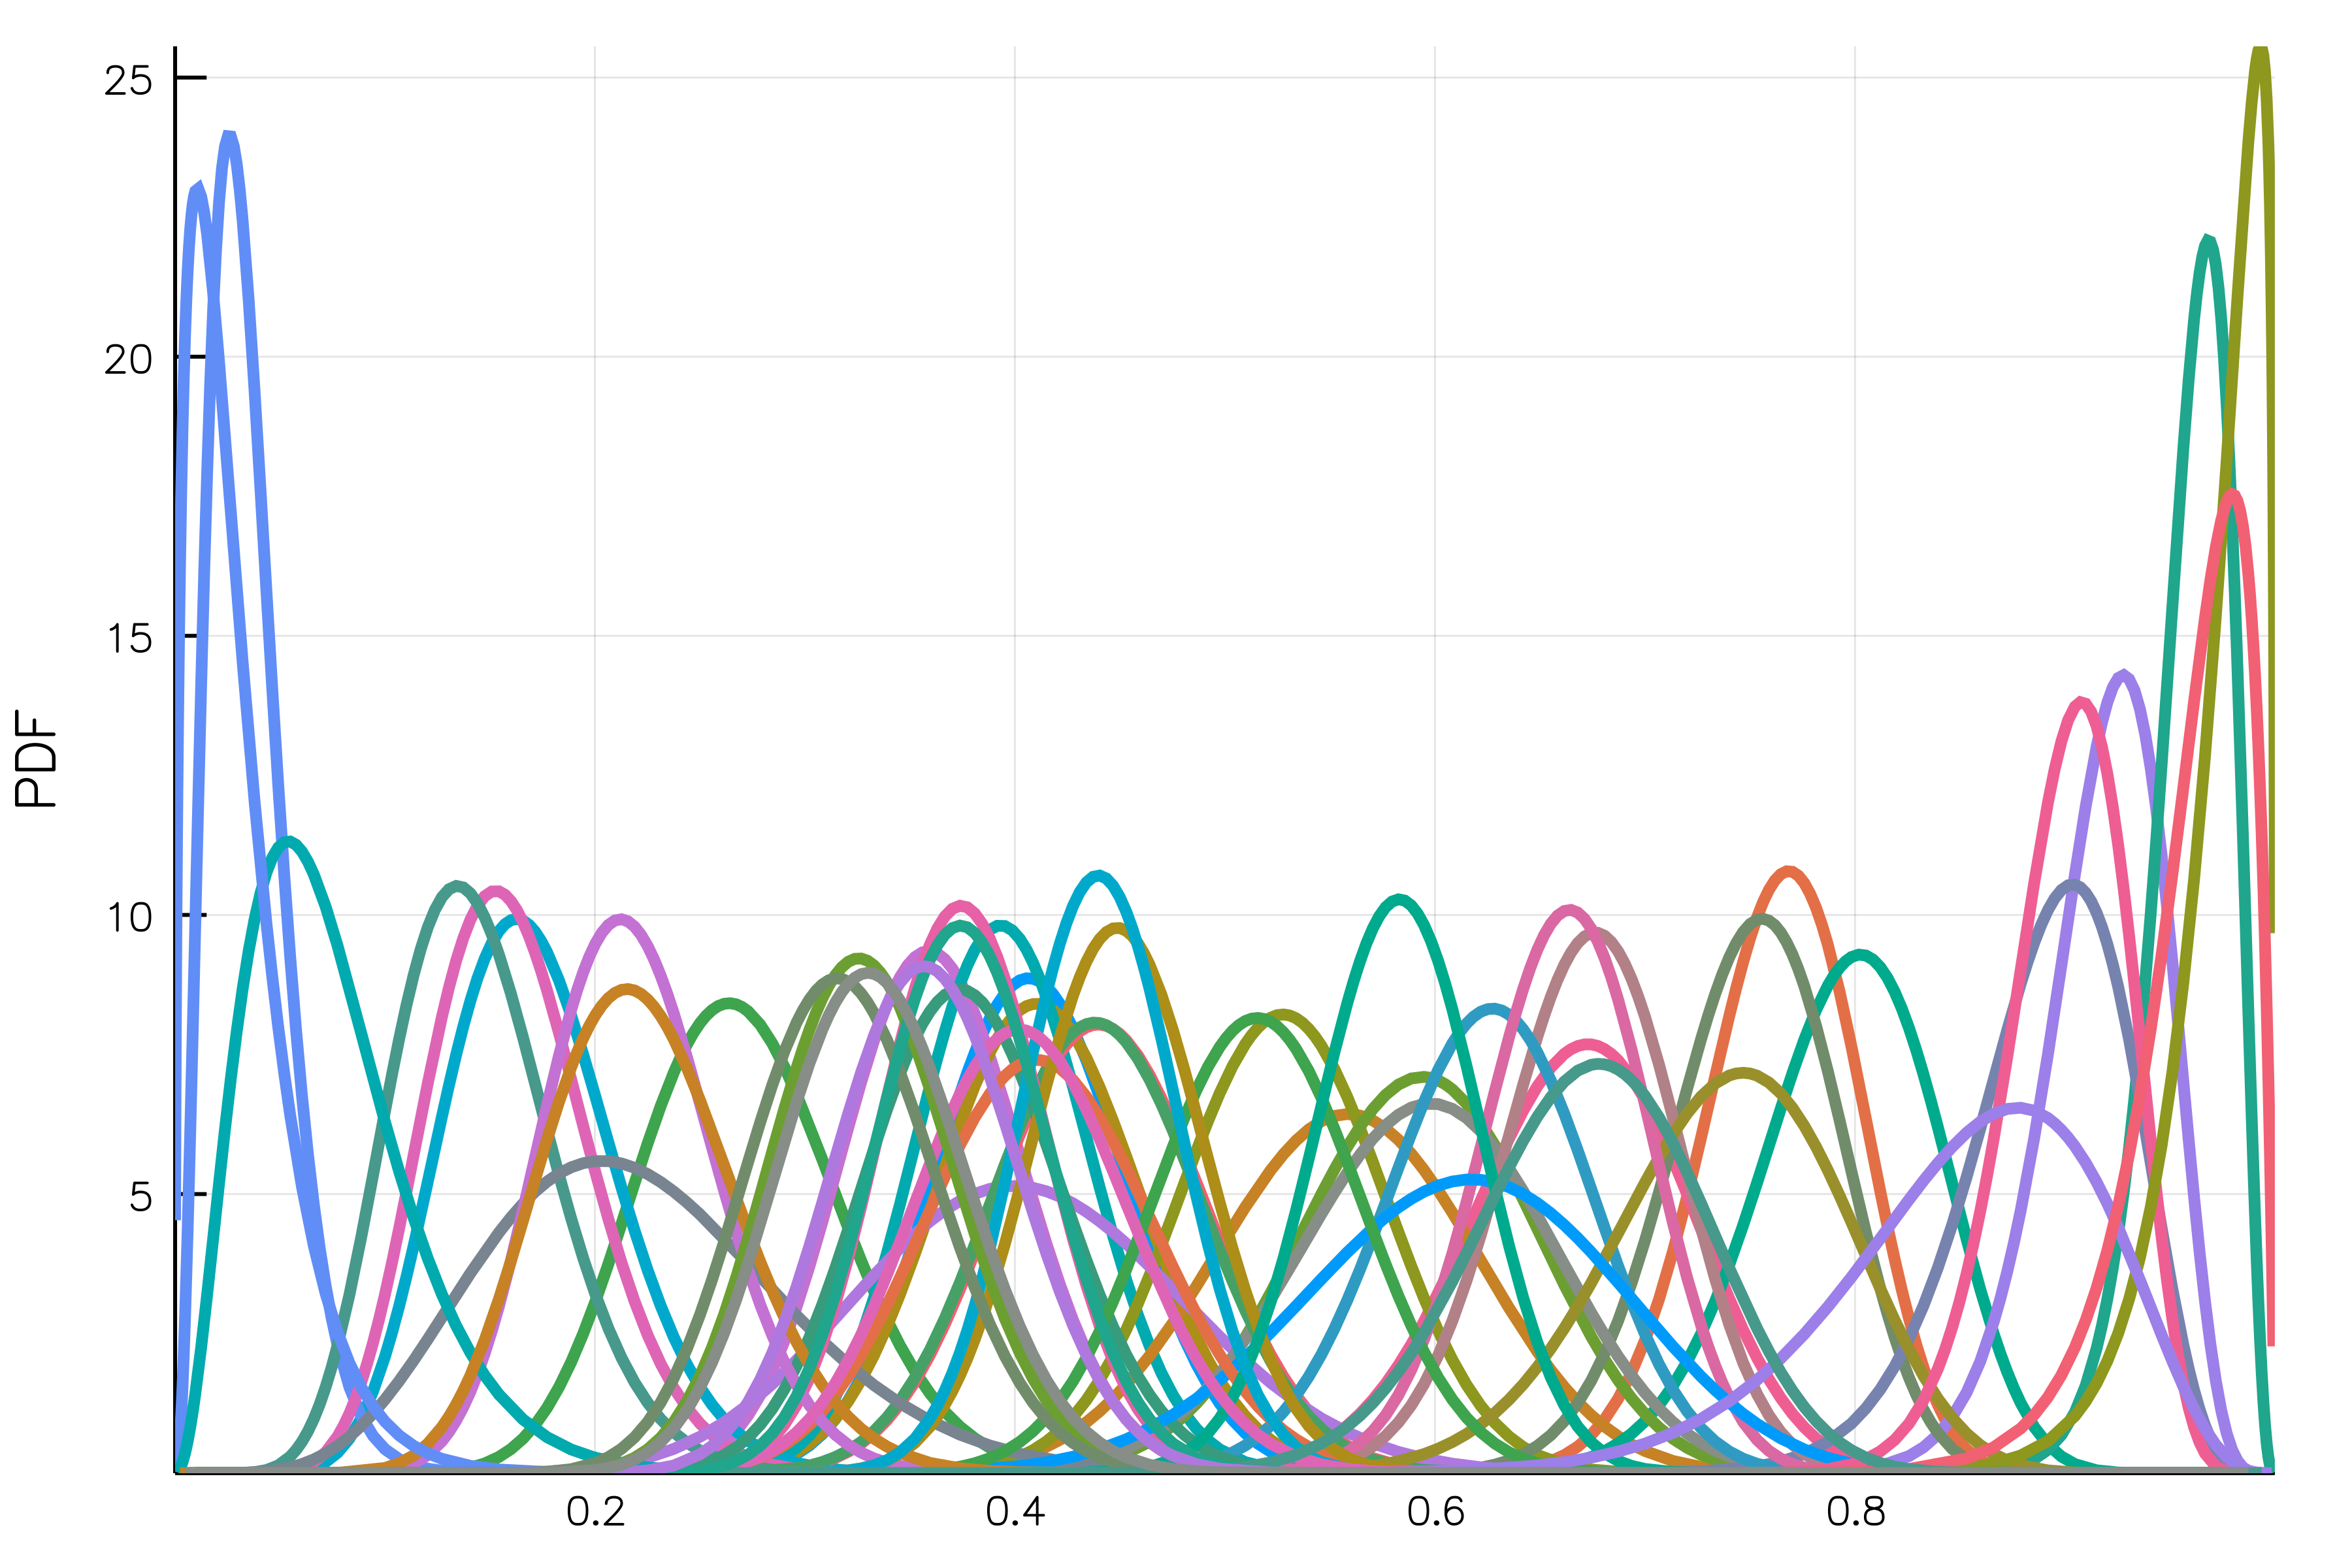
\includegraphics[width=\textwidth]{ims/beta100.png}
  \caption{Distribuições Beta para 50 agentes}
  \label{fig:betas100}
\end{figure}


A cada iteração da simulação um dos agentes vai ser escolhido e vai interagir
com um de seus vizinhos, a princípio num grafo completo imposto exogenamente
(estabeleço na condição inicial quais os vizinhos). A interação é assim em
díades, assíncrona (os agentes atualizam seus atributos em momentos distintos) e
sequencial (um agente atualiza por vez) \cite{wilensky2015introduction}. A
dependência dos resultados em relação ao número de agentes e de crenças vai ser
explorada. Estamos interessados nas alterações ao longo prazo (em termos de
iterações) da configuração dos \(x\) sob diferentes combinações de parâmetros,
tendo em vista as interações dos agentes \cite{acemoglu2011opinion}
\footnote{Como vamos definir longo prazo e analisar o modelo é tema da seção
  metodológica.}.

Quando os agentes interagem \(i\) atualiza sua opinião em alguma\footnote{Qual
  questão vão ``debater'' vai ser definido por meio de um sorteio sem viés. Uma
  outra implicação possível, a ser adicionada em trabalhos futuros, é considerar
  um viés nessa seleção, o que representaria saliência no sentido dado por
  \citeonline{zaller1992simple}: qual questão os agentes estão dando atenção,
  isto é, qual questão está mais acessível na memória deles.} questão segundo as
equações 2.3 e 2.4. Dado que os agentes agora tem um conjunto de opiniões é
plausível considerar que um conjunto de agentes tenham determinadas opiniões em
que eles tenham maior certeza, identificação, ou centralidade para o seu perfil
ideológico. Sendo assim na condição inicial alguma proporção de agentes tem uma
questão no seu perfil \(I\) cujos \(\sigma\) associados são aproximadamente zero. Com
isso buscamos analisar o papel de agentes ``inflexíveis'' na dinâmica
populacional. A proporção de agentes intransigentes ou inflexíveis é assim um
parâmetro da simulação.

Os agentes também vão reconsiderar suas opiniões e certezas sobre as questões
segundo uma probabilidade \(\rho\). Do ponto de vista teórico, estamos considerando
a possibilidade de fatores não relacionados à influência social levarem o agente
a mudar seu posicionamento sobre questões \cite{flache2017, lorenz2017modeling}.
Do ponto de vista metodológico, \citeonline{macy2015signal} argumenta que
pequenas perturbações no comportamento local dos agentes pode levar a mudanças
drásticas nas propriedades sistêmicas. Particularmente, consideram que adicionar
ruído pode: eliminar equilíbrios frágeis, o que reduz o conjunto de resultados e
tornando-os mais previsíveis; e embora aumente a heterogeneidade local isso pode
acabar facilitando interações sociais que reduzem a diversidade global
\cite[p.323]{macy2015signal}. A nova opinão é sorteada independentemente da
opinião anterior do agente. Contudo, no caso em que o agente seja intransigente
na questão ele não será sujeito ao efeito do ruído.


\section{Parâmetros-Chave}

Os parâmetros-chave para configuração e inicialização do modelo, cujos valores
seguem \citeonline{martins2008continuous}, \citeonline{deffuant2000mixing} e
\citeonline{lorenz2017modeling}, são:

\begin{itemize}
\item A população de \(500 < N < 5000\) agentes;
\item O número de questões \(1 \leq \text{n\_issues} \leq 10\); 

\item As incertezas \(0.01 \leq \sigma_i \leq 0.5\);
  \begin{itemize}
  \item Agentes intransigentes vão ter uma de suas opiniões com incerteza
    próxima a zero (\(1e-15\));
  \end{itemize}

\item O parâmetro de confiança \(0.1 \leq p \leq 0.99\);
  
\item A proporção de agentes intransigentes \(0.0 \leq (\text{p\_intran}) \leq 0.1\);

\item A probabilidade de reconsideração \(0.0 \leq \rho  \leq 0.1\);
  
\end{itemize}

\section{Inicialização e Iteração}

A inicialização da simulação depende dos parâmetros-chave apresentados. Na
condição inicial temos uma população de \(N\) agentes, que tem por atributos: um
conjunto de pares \(I_i = ((o_{i,1},\sigma_{i,1}^2), \ldots, (o_{i,n},\sigma_{i,n}^2))\), onde
o número de questões, \(n\), é uma variável global, cada \(o\) é retirado de uma
distribuição Beta(\(\alpha,\beta\)), onde cada agente tem um \(\alpha\) e um \(\beta\) próprio,
com valores\footnote{Paramêtros com valores \(\leq\) 1 ou geram distribuições de
  formato uniforme, quando \(\alpha = \beta = 1.0\), ou com formato de U. Quanto ao
  limiar superior, o valor de 100 permite que tenhamos agentes com distribuições
  centralizadas em ambos os extremos, dado que a média \(\mu\) é dada por
  \(\frac{\alpha}{\alpha + \beta}\), de forma que a média mínima é 0.011.} entre 1.1 e 30; o
\(\sigma^2\) é uma variável global ; um posicionamento ideológico, ou ponto ideal,
\(x_i = \frac{1}{n} \sum_{k = 1}^n o_{i,k} \); e um conjunto de vizinhos, o qual
depende de qual a rede os agentes estão. Uma determinada proporção de agentes,
contudo, vai ter um \(\sigma_i = (1e-15 ) \approx 0.0 \). Qual em particular é sorteado de
seu \(I\). Quantos agentes são intransigentes é dado por \(\text{p\_intran}\).

 Uma iteração da simulação, a
passagem de digamos \(t=2\) para \(t=3\), é dada pela aplicação de dois
procedimentos: a atualização via influência social e a atualização aleatória.
Uma repetição da simulação é a aplicação iterativa desses dois procedimentos ao
longo de um tempo \(t \).

O procedimento de influência social é o seguinte: escolhemos um agente \(i\) da
população. Então escolhemos um de seus vizinhos, \(j\). Sorteamos uma das
questões \(k \in (1,\ldots,n)\), e logo em seguida selecionamos os
\((o_{i,k},o_{j,k})\) e \((\sigma_{i,k}^2,\sigma_{j,k}^2)\) correspondentes à questão. A
partir daqui temos duas opções, \(i\) atualiza \(o_{i,k}\) segundo as equações
2.3 e 2.4. Essa regra é um parâmetro global da simulação, o que significa que a
cada repetição todos os agentes atualizam suas crenças segundo a mesma regra.

Ademais, temos o ruído. Novamente escolhemos um agente \(i\) da população.
Sorteamos uma questão e selecionamos \(o\) e \(\sigma^2\) correspondentes. Se o
agente é intransigente naquela questão então ele não muda de opinião. Sorteamos
um \(\xi\) retirado de uma distribuição uniforme \(U([0,1])\) e se \(\xi < \rho\) \(i\)
muda \(o\) para um valor retirado de outra distribuição uniforme (U[0,1]). Os
\(x_i\), o objeto de interesse de análise, são atualizados sempre que ocorrerem
mudanças nas crenças dos agentes.

\section{Metodologia de Análise}

Dentre as diversas formas de analisar um ABM a análise de sensibilidade global
se destaca como uma forma de ter uma compreensão ampla, geral, do comportamento
do modelo \cite{north2007managing}. O primeiro passo da análise envolve, então,
 ter uma compreensão geral do comportamento do modelo para então passarmos
para regiões particulares do espaço de parâmetros.

Contudo, o alto custo computacional de varrer esse espaço de parâmetros faz com
que só seja possível realizarmos uma análise global, na maioria dos casos, se
seguirmos métodos formais da literatura de análise de sensibilidade
\cite{railsback2012agent}. Esses métodos trazem o benefício de determinar como
selecionar subconjuntos de todas as combinações de parâmetros, reduzindo o
número de realizações necessárias da simulação e de trazerem formas sistemáticas
de interpretar os resultados \cite{railsback2012agent}.

Quanto à amostragem uma estratégia comum são as parametrizações de Monte Carlo:
sortear valores de parâmetros usados para as realizações das simulações a partir
de distribuições uniformes nos intervalos de valores dos parâmetros
\cite{laver2011party}. O problema dessa estratégia é que o espaço de parâmetros
não é coberto igualmente, havendo a possibilidade de pontos de acumulação ou
espaços vazios \cite{pereda2017brief}.

\citeonline{saltelli2008global} argumenta que para manter uma dispersão equitativa
dos pontos no espaço de parâmetros é necessário um algoritmo que enviese a
seleção de novos pontos para mantê-los afastados dos pontos já presentes. Desta
forma vamos usar o método de Saltelli de amostragem, dado que garante a partição
equitativa do espaço de parâmetros \cite{herman2017salib}. Especificamos então
um \(n\) base a partir do qual o ``sampler'' gera n * (2d + 2), onde \(d\) é o
número de parâmetros. No nosso caso \(d = 6\), pois vamos ter como parâmetros :
N (população), número de questões (codificado como n\_issues ), \(p\), \(\sigma\), a
proporção de agentes intransigentes (codificado como p\_intran)
\(\rho\). Para garantir um coeficiente de erro baixo no cálculo
subsequente dos índices de sensibilidade especificamos um \(n\) base de
\(5000\), de forma que rodamos \(70.000\) parametrizações.


\begin{figure}[h]
    \centering
    \begin{subfigure}[b]{0.49\textwidth}
      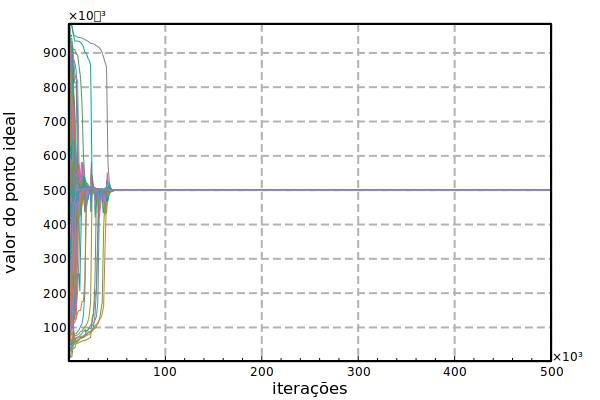
\includegraphics[width=\textwidth]{ims/timeseries1.png}
      \caption{\( \sigma = 0.1\) }
    \end{subfigure}
    \begin{subfigure}[b]{0.49\textwidth}
      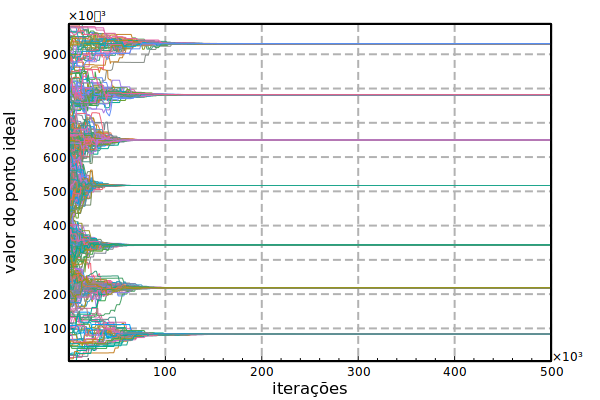
\includegraphics[width=\textwidth]{ims/timeseries2.png}
       \caption{\(\sigma = 0.02\) }
      \end{subfigure}
      \caption{Evolução dos pontos ideais dos agentes ao longo de duas realizações.
        Parametrização: \(  N = 500, p = 0.9, \rho = 0.0, n\_issues = 1 , p\_intra
        n= 0.0 \)}
      \label{fig:tseries1}
    \end{figure}
    
    Uma vez especificado o método de amostragem especificamos uma medida do
    sistema para que possamos analisá-lo \cite{railsback2012agent}. Escolhemos o
    desvio padrão dos pontos ideais após \(1.000.000\) iterações como output
    para análise\footnote{Testamos diversas parametrizações com n\_issues \(=
      1\) e observamos que a partir de \(50.000\) iterações a implementação
      replica os resultados de \citeonline{martins2009bayesian}.}, dado que nos
    diz o quão concentrados/dispersos são os pontos ideais da população. Uma
    outra opção de medida do sistema seria o número de opiniões finais distintas
    após as iterações, o que nos daria uma medida de ``cobertura'' do sistema:
    uma maior cobertura implicaria num número maior de posicionamentos distintos
    \cite{bramson2016disambiguation}. Contudo, teríamos que estabelecer um \(N\)
    base, pois de outra forma esse parâmetro explica quase que totalmente o
    valor do output a ser analisado pela análise de sensitividade.

    No primeiro gráfico da figura \ref{fig:tseries1} temos um desvio padrão
    próximo zero, e um único posicionamento ideológico final. Já no segundo
    gráfico precisaríamos arredondar os pontos ideais finais, para entre 1 e 6
    casas decimais, para chegarmos a conclusão que existem cerca de 6 pontos de
    convergência. Se não arredondarmos o resultado final teríamos uma medida
    próxima de 500 pontos ideais, e que não nos informaria a respeito da
    cobertura do sistema. Já o desvio padrão nos indica a dispersão dos pontos
    ideais, pois tem valor de aproximadamente 0.24, próximo ao da condição
    inicial. Um outro problema do uso do número final de pontos ideais ao fim de
    uma realização é que a medida não é robusta a ruídos ou proporções de
    agentes intransigentes diferentes de 0. Quando há ruído ou agentes
    intransigentes o número final de pontos ideais não informa muito sobre a
    dinâmica do sistema. Na Figura \ref{fig:nonnullrho} temos um comportamento
    qualitativamente similar ao da Figura \ref{fig:tseries1} (b), mas o número
    de opiniões finais é próximo de 500 \footnote{Isso envolve inclusive se
      medirmos o número de pontos ideais finais com valores arredondados.
      Arredondar demais faz com que perdamos a comparabilidade com a condição
      inicial, que passa a não ter mais 500 pontos ideais. No caso da figura
      \ref{fig:nonnullrho} usar o número de pontos ideais distintos como medida
      nos informa que há grande cobertura no sistema, mas passaria dispercebido
      o fato de que ao fim o comportamento é bastante similar ao caso com ruído
      nulo. A dispersão não nos informa sobre a existência dos ``clusters'', mas
      ao menos mantêm a consistência nos casos com e sem ruído.}.
    
  \begin{figure}[H]
    \centering
    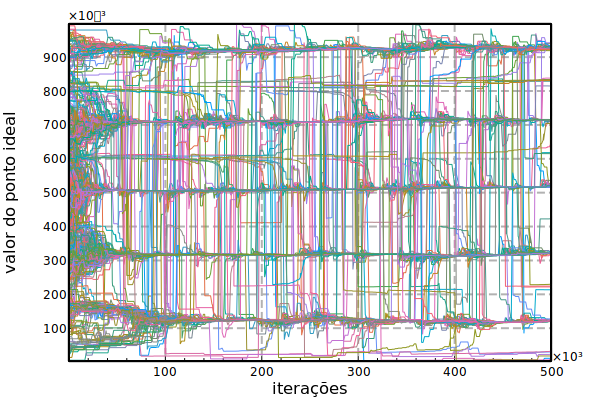
\includegraphics[width =10cm]{ims/ts5.png}
    \caption{Parametrização equivalente a Figura \ref{fig:tseries1} (b),
      mas com \(\rho = 0.001\).}
    \label{fig:nonnullrho}
  \end{figure}

  
Para a análise, seguimos \citeonline{ten2016sensitivity} e combinamos
histogramas da medida do sistema, gráficos de dispersão e índices de
sensibilidade.Os índices de sensibilidade utilizados são os índices de
Sobol\footnote{Tanto a amostragem quanto a análise de sensibilidade são feitas
  usando o pacote de Python SALib \cite{herman2017salib}.}, particularmente
índices de Sobol de primeira ordem e totais \cite{saltelli2008global}. Os
índices de Sobol decompõem o impacto dos parâmetros na variância do
\textit{output} de interesse. Os índices de primeira ordem incluem contribuições
lineares e não-lineares dos parâmetros, mas não efeitos interativos
\cite{ten2016sensitivity}. Já índices totais incluem todos os efeitos de ordem
maior decorrentes das interações entre os parâmetros \cite{saltelli2008global}.

\section{Resultados}

Rodamos então \(70.000\) parametrizações por \(1.000.000\) de iterações tendo
por \(Y\), o \textit{output} de interesse, o desvio padrão  dos pontos ideais da
população (\(\text{Ystd}\)) após as iterações. São \(6\) os parâmetros de input
: o número de agentes (\(N\)), o número de questões (\(\text{n\_issues}\)), o
parâmetro de confiança (\(p\)), a incerteza (\(\sigma\)),  o ruído \(\rho\), e a
proporção de agentes intransigentes (\(p\_intran\)) nos
limiares apresentados na seção Parâmetros-Chave.

Como uma primeira aproximação do comportamento geral do modelo, a Figura
\ref{fig:hists1} apresenta a dispersão dos pontos ideais na condição inicial e
ao fim das simulações para cada parametrização.

\begin{figure}[h]
    \centering
    \begin{subfigure}[b]{0.49\textwidth}
      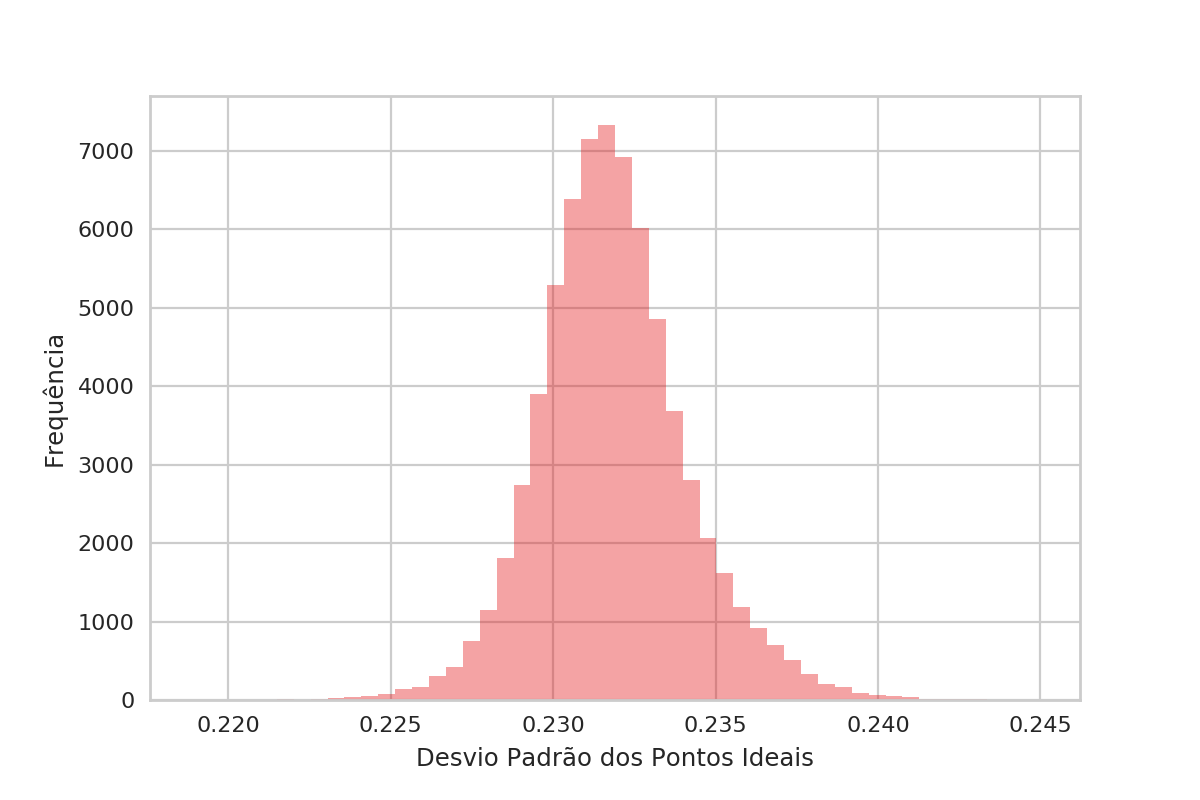
\includegraphics[width=\textwidth]{ims/diststdinit.png}
      \caption{Condição inicial}
    \end{subfigure}
    \begin{subfigure}[b]{0.49\textwidth}
      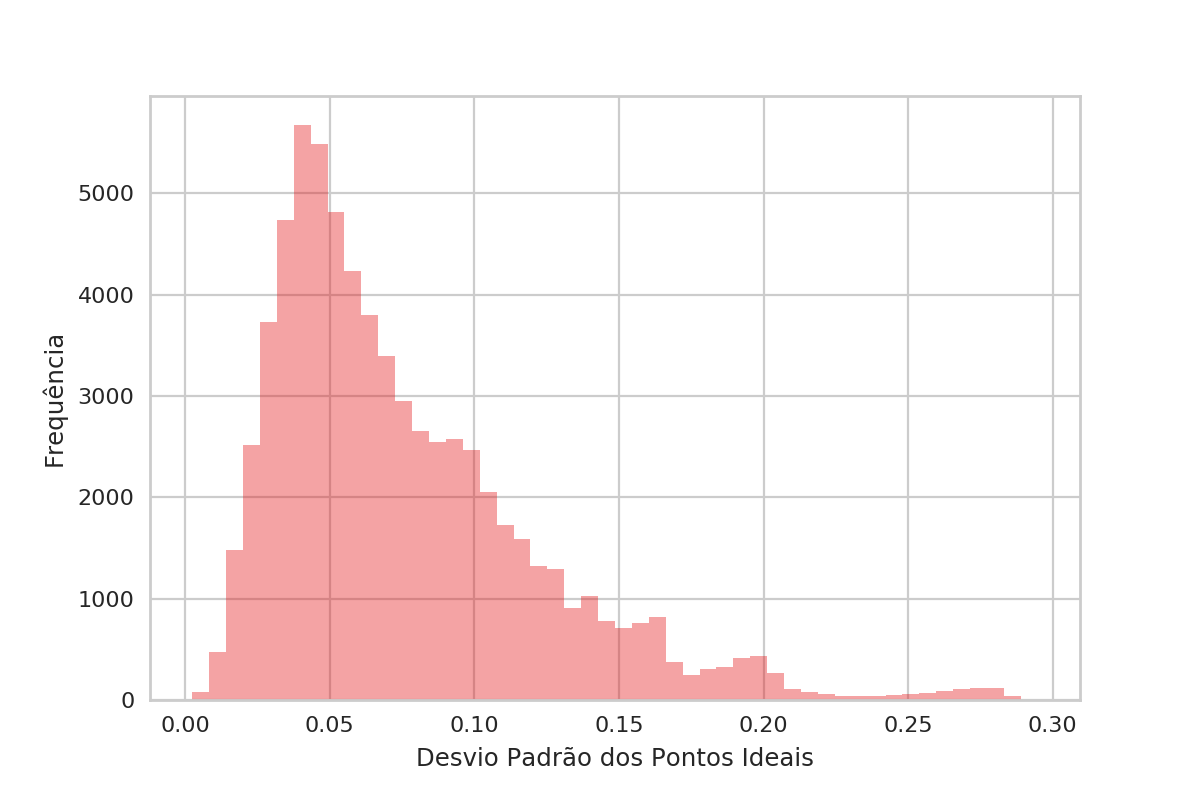
\includegraphics[width=\textwidth]{ims/distY.png}
       \caption{Após 1.000.000 iterações}
      \end{subfigure}
      \caption{Desvio padrão dos pontos ideais das populações para cada parametrização}
      \label{fig:hists1}
    \end{figure}
    

%
%
%\begin{figure}[H]
%  \centering
%  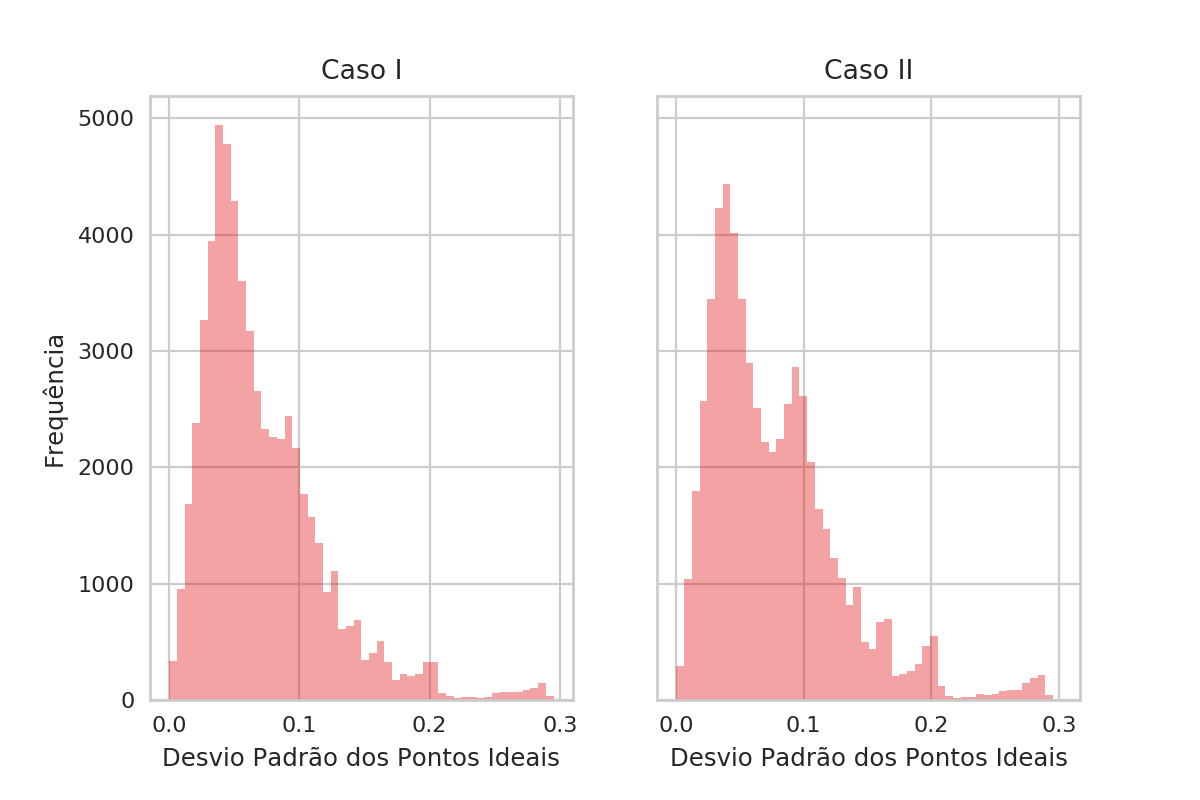
\includegraphics{ims/distYs.png}
%  \caption{Output (desvio padrão dos pontos ideais) }
%  \label{fig:Yshist}
%\end{figure}

    A Figura \ref{fig:hists1} nos leva a interpretar que a aplicação iterativa
    do procedimento do modelo, deixa a distribuição de opiniões menos dispersa,
    com uma maior concentração das parametrizações em outputs de baixa dispersão
    (entre 0.0 e 0.1). Isso condiz com as regras de atualização (assimilativa,
    mas na qual agentes distantes tem pouco impacto na opinião um dos outros) e
    com o fato dos agentes terem por vizinhos todos os outros agentes. Isto é,
    os agentes ao interagirem ou ficam mais parecidos ou não são influenciados.
    O modelo tem assim uma forte tendência assimilativa, ao menos num grafo
    completo. Contudo, a figura não nos informa qual parâmetro é responsável por
    isso, ou quais os valores de concentração (centrais ou extremos).

    A primeira pergunta pode começar a ser respondida por meio de gráficos de
    dispersão. A partir da Figura \ref{fig:scatter1} podemos inferir que há uma
    relação negativa entre os parâmetros \(\text{n\_issues}, p, \sigma \) e a
    dispersão dos pontos ideais (\( \text{Ystd}) \). A relação entre \(p\) e
    \(\sigma\) são explicadas pelo fato de agentes que ``confiam'' mais na opinião
    dos outros agentes e são mais incertos vão convergir mais rápido para a
    mesma opinião.

\begin{figure}[H]
    \centering
    \begin{subfigure}[b]{0.49\textwidth}
        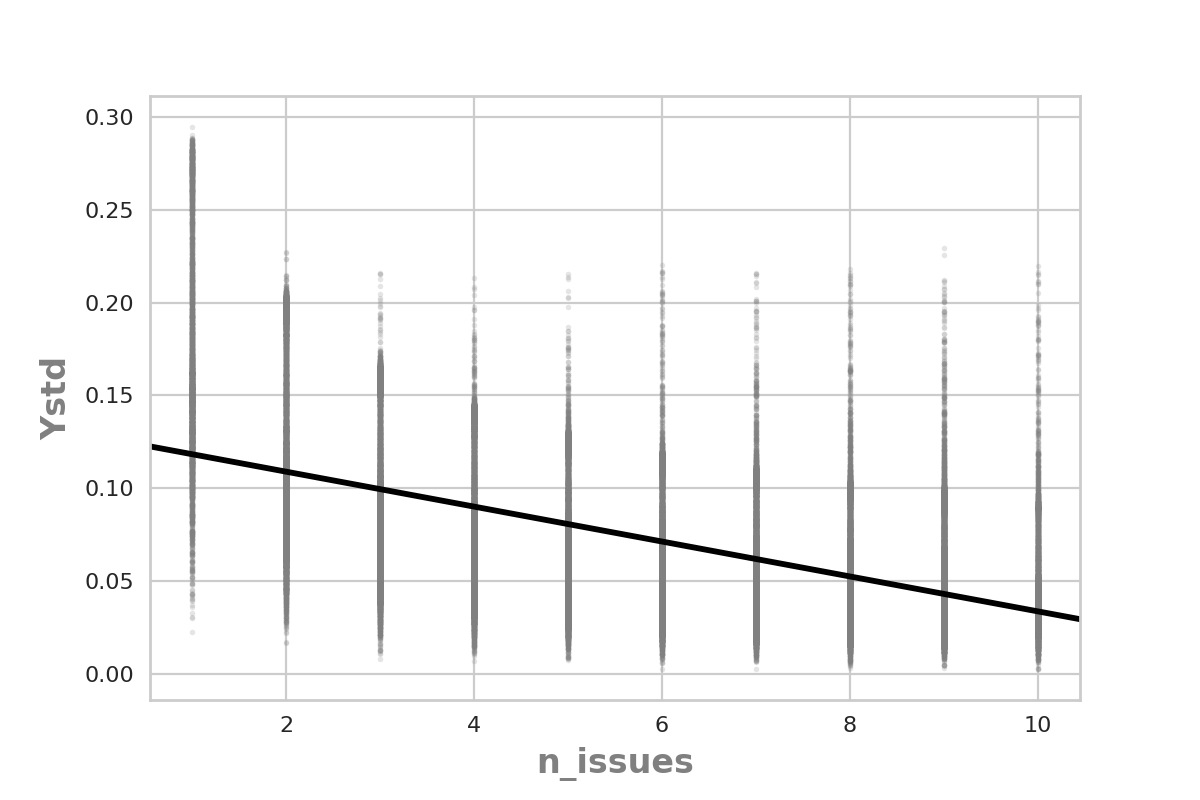
\includegraphics[width=\textwidth]{ims/mutoregressions/regressionmutatingon_issues.png}
    \end{subfigure}
    \begin{subfigure}[b]{0.49\textwidth}
        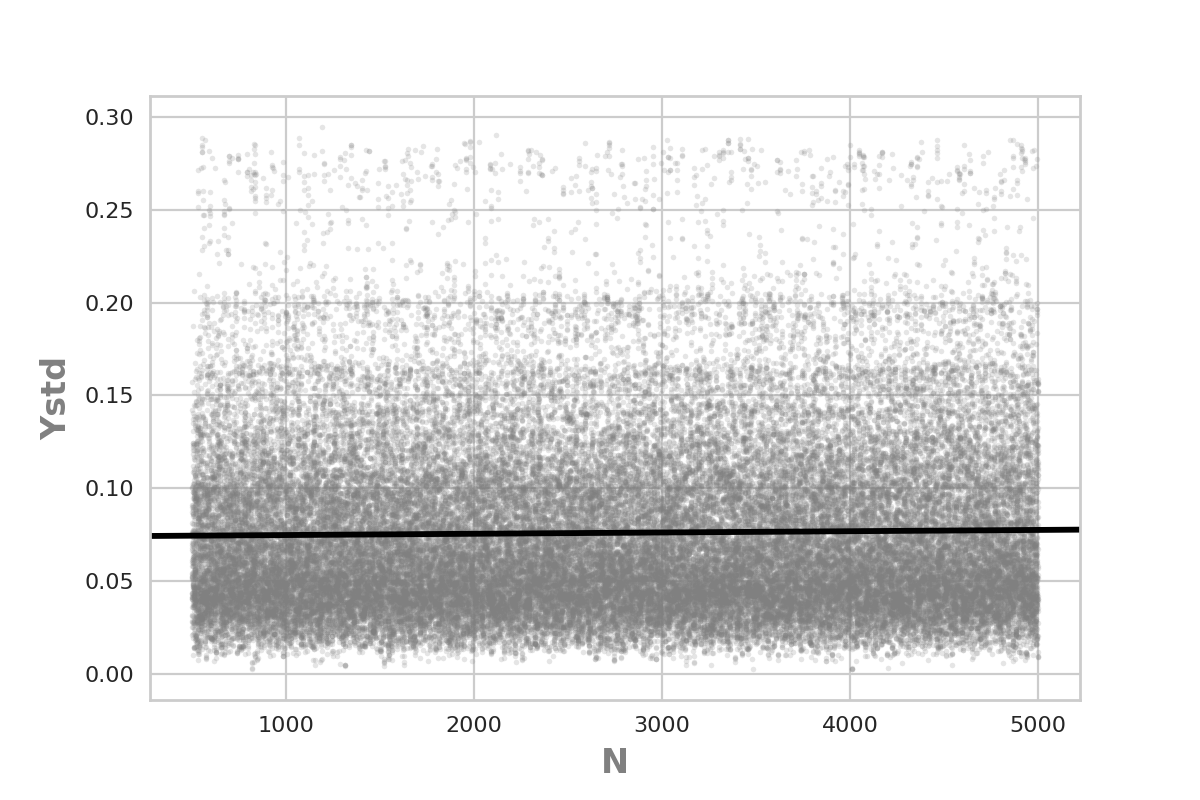
\includegraphics[width=\textwidth]{ims/mutoregressions/regressionmutatingoN.png}
    \end{subfigure}

    \begin{subfigure}[b]{0.49\textwidth}
        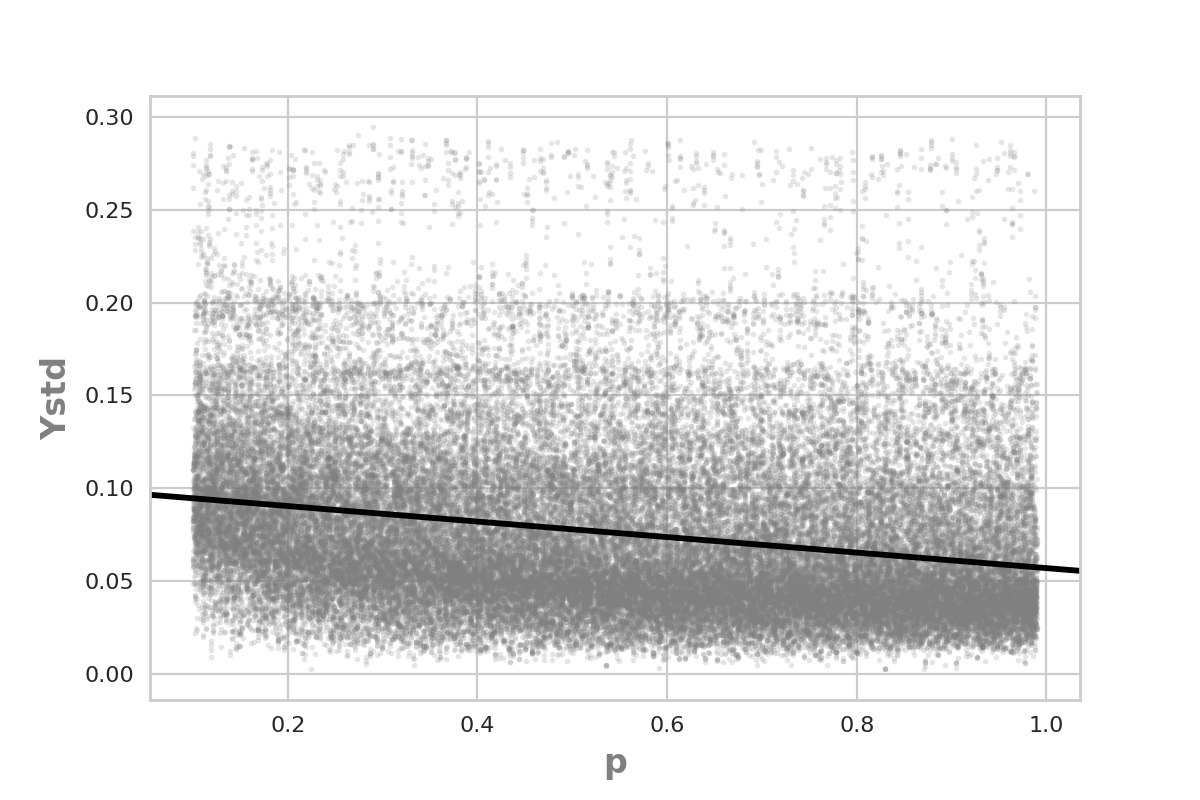
\includegraphics[width=\textwidth]{ims/mutoregressions/regressionmutatingop.png}
      \end{subfigure}
          \begin{subfigure}[b]{0.49\textwidth}
            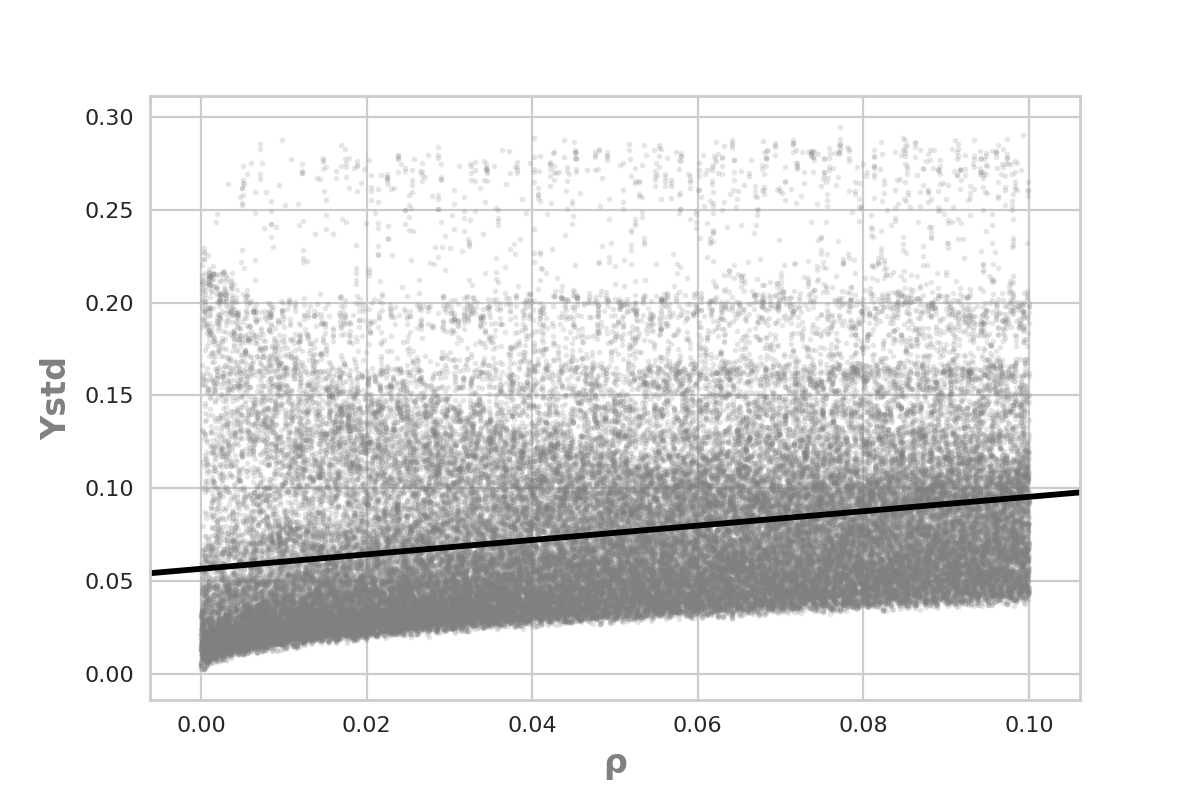
\includegraphics[width=\textwidth]{ims/mutoregressions/regressionmutatingorho.png}
      \end{subfigure}

                \begin{subfigure}[b]{0.49\textwidth}
            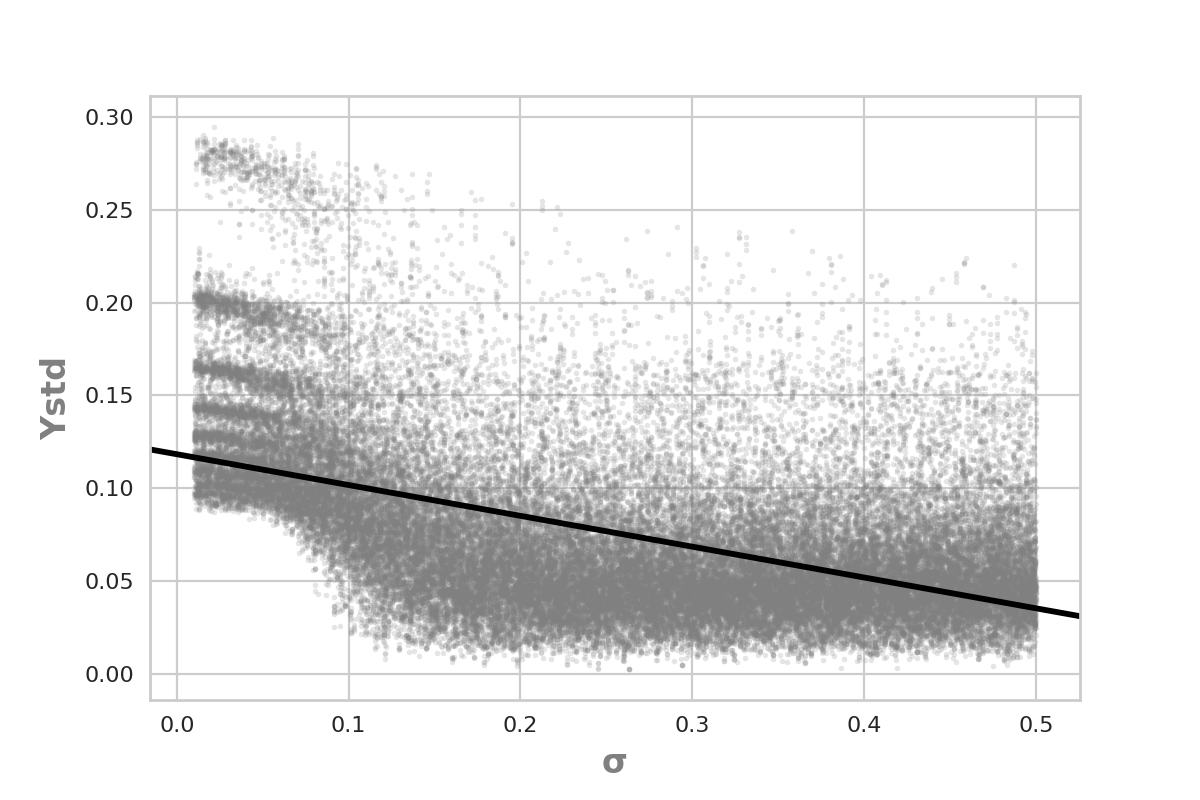
\includegraphics[width=\textwidth]{ims/mutoregressions/regressionmutatingosigma.png}
          \end{subfigure}
                \begin{subfigure}[b]{0.49\textwidth}
            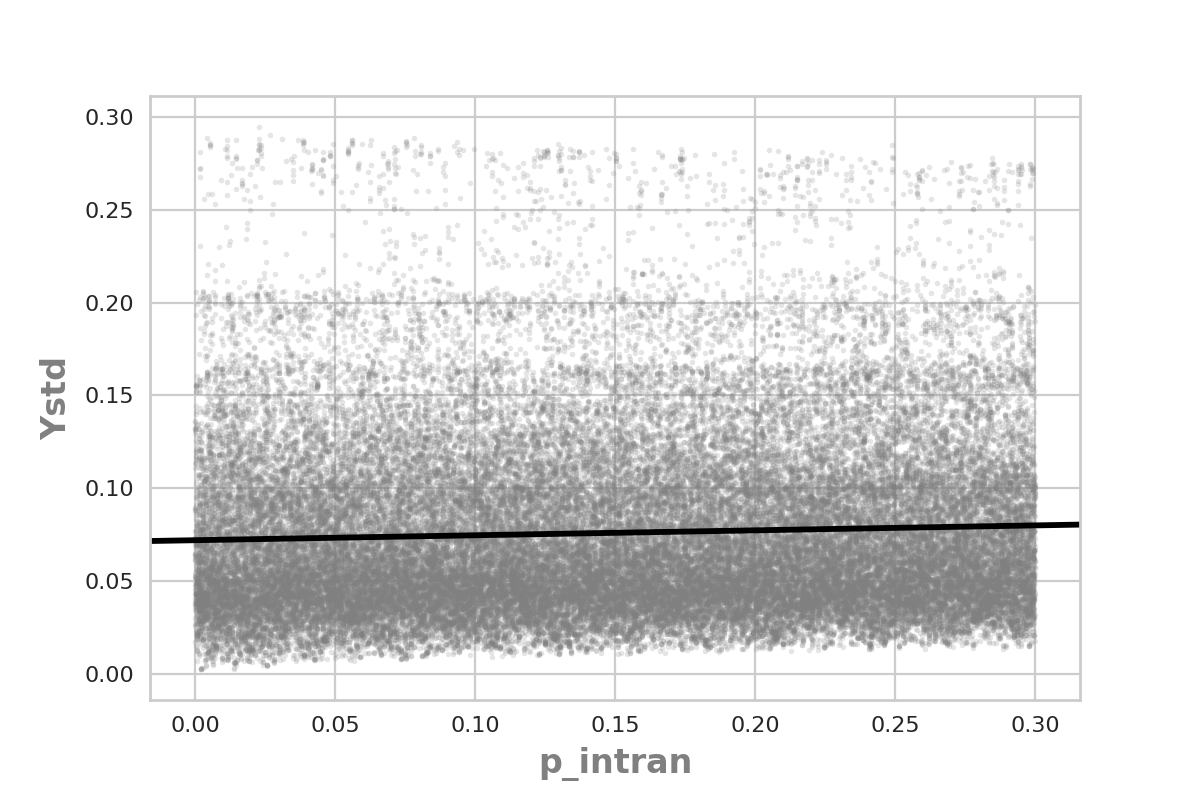
\includegraphics[width=\textwidth]{ims/mutoregressions/regressionmutatingop_intran.png}
    \end{subfigure}
    \caption{Gráfico de dispersão para 70.000 parametrizações.}
    \label{fig:scatter1}
    Fonte:Elaboração própria.
\end{figure}

O parâmetro \(\rho\), o ruído, por sua vez, tem uma relação positiva com a
dispersão do sistema. Interessante notar, contudo, que o tamanho da população
parece não ter relação com o desvio padrão dos pontos ideais da população.

A intensidade dos parâmetros na variância da medida do sistema (Ystd) fica mais
claro na Figura \ref{fig:sobol1}:

\begin{figure}[H]
  \centering
  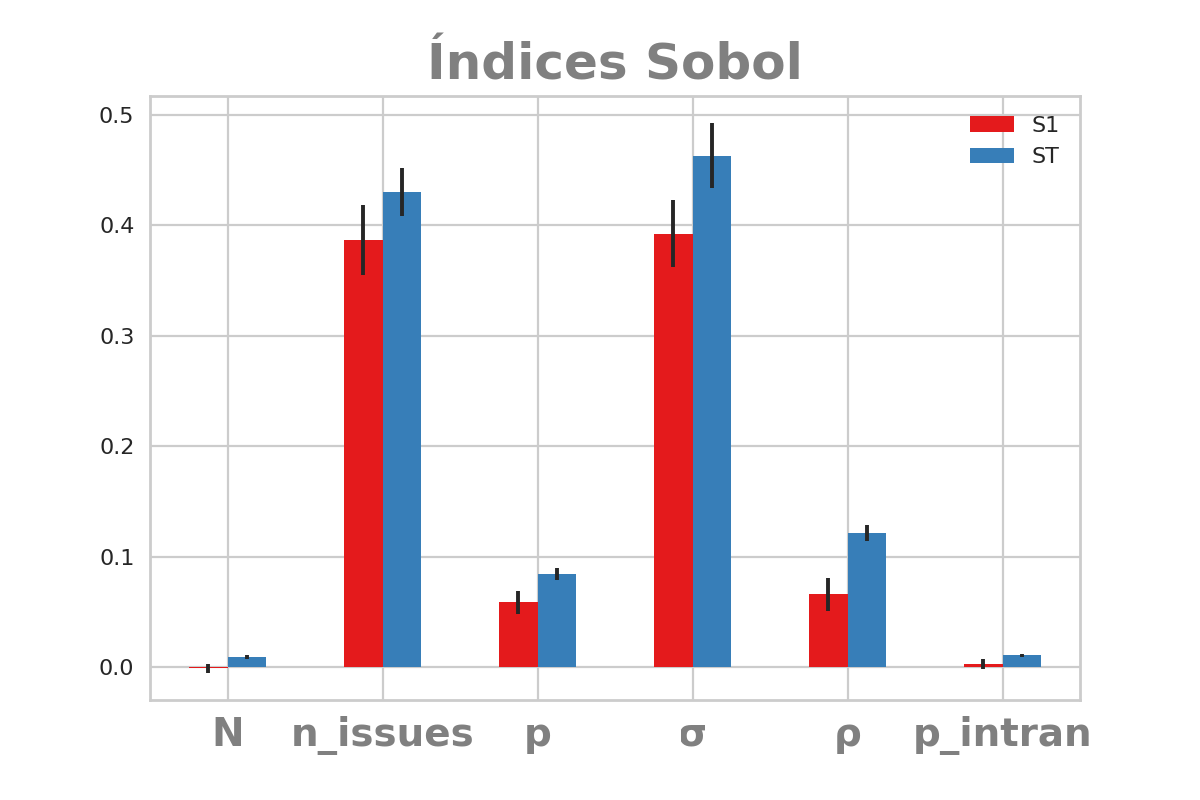
\includegraphics{ims/barplotmuto5k.png}
  \caption{Índices de Sobol de sensibilidade}
  \label{fig:sobol1}
\end{figure}

Como mostra a Figura \ref{fig:sobol1} o parâmetro \(N\) não tem impacto sobre a
variância de \(Ystd\), de forma que podemos tratá-lo como uma constante para
análise subsequentes. A figura mostra que a maior parte da variância na
dispersão dos pontos ideais pode ser explicada pelos parâmetros \(\sigma\) e
\(\text{n\_issues}\). Além disso há pouca diferença entre os índices de primeira
ordem e os índices totais, o que implica que há poucos efeitos interativos entre
os parâmetros. Ademais, os coeficientes de erro são pequenos\footnote{Para os
  valores precisos ver o Apêndice.} tendo em vista que a análise foi feita a
partir de 70.000 parametrizações selecionadas por meio do método de Saltelli.

Um resultado contra-intuitivo, contudo, é o baixo valor de impacto do parâmetro
\(p\_intran\). A comparação entre as figuras \ref{fig:tseries1} e
\ref{fig:tseries2} sugere que esse resultado seja um artefato da medida Ystd.

\begin{figure}[H]
    \centering
    \begin{subfigure}[b]{0.49\textwidth}
      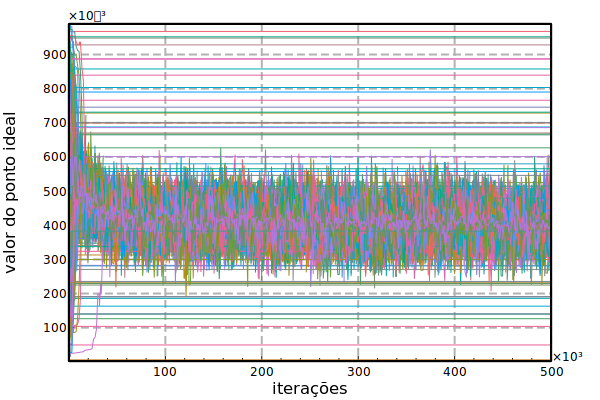
\includegraphics[width=\textwidth]{ims/timeseries3.png}
      \caption{\( \sigma = 0.1\) }
    \end{subfigure}
    \begin{subfigure}[b]{0.49\textwidth}
      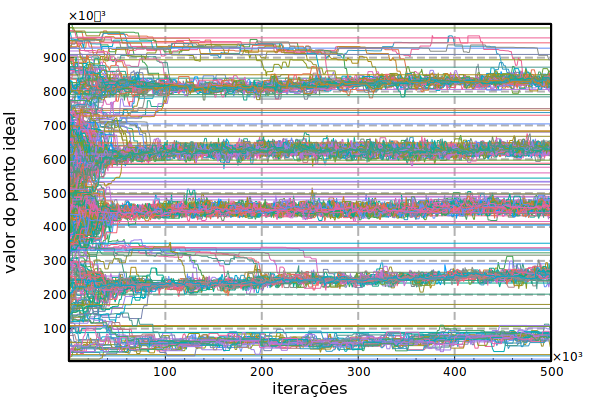
\includegraphics[width=\textwidth]{ims/timeseries4.png}
       \caption{\(\sigma = 0.02\) }
      \end{subfigure}
      \caption{Evolução dos pontos ideais dos agentes ao longo de duas realizações.
        Parametrização: \(p\_intran = 0.15, \text{ } N = 500,  \text{ }   p =
        0.9,  \text{ }  \rho = 0.0,  \text{ }  n\_issues = 1 \)}
      \label{fig:tseries2}
    \end{figure}
    
    Enquanto que na figura \ref{fig:tseries1} (a) o sistema converge para um
    único valor, na figura \ref{fig:tseries2} a população oscila no espaço ao
    redor desse valor. As figuras \ref{fig:tseries1} e \ref{fig:tseries2} (b)
    exibem uma diferença equivalente de comportamento. O parâmetro parece assim
    ter impacto sobre a dinâmica, particularmente sobre a cobertura. Quais
    agentes são intransigentes é aleatório, mas como eles não mudam de opinião
    em um determinado tema é de se esperar que acabem por atrair os outros
    agentes para sua posição. Para testar a intuição de que os agentes
    intransigentes enviesam a dinâmica para a posição deles testamos a mesma
    parametrização que a figura \ref{fig:tseries2} (a), mas com os \(15\%\)
    intransigentes localizados entre os valores maiores que 0.8 ou menores que
    0.2 no espectro ideológico. A figura \ref{fig:tseries3} demonstra que a
    atração para onde existem mais agentes intransigentes realmente
    ocorre\footnote{Com a figura \ref{fig:tseries3} replicamos o comportamento
      do modelo de \citeonline{deffuant2002can}.}.

      \begin{figure}[H]
    \centering
    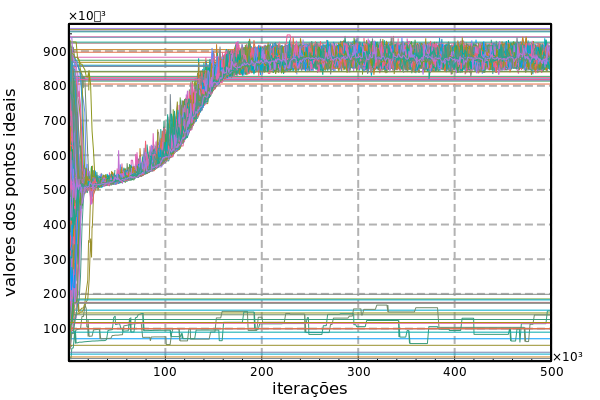
\includegraphics[scale=0.7]{ims/sigma01extremes.png}
    \caption{ Evolução dos pontos ideais dos agentes sob efeito de
      intransigentes nos extremos. Parametrização: \(p\_intran = 0.15, \text{ }
      N = 500, \text{ } p = 0.9, \text{ } \rho = 0.0, \text{ } n\_issues = 1 \)}
    \label{fig:tseries3}
  \end{figure}
  

    Como nem o desvio padrão nem o número de pontos ideais finais,
    como discutido anteriormente, nos dão medidas quantitativas desse impacto
    passamos a uma análise gráfica de certas combinações de parâmetros típicas.
    Os gráficos de dispersão nos indicam\footnote{Regressões polinomiais de
      terceira ordem foram usadas para auxiliar essa análise. Estão no
      apêndice.} possíveis restrições aos limiares dos parâmetros.

    Dado o pequeno impacto de \(N\) e \(p\) vamos os manter constantes, com
    valores de 500 e 0.9 respectivamente. Uma conjunto de parametrizações não
    abarcado pela análise de sensibilidade global é quando \(p\_intran = \rho  =
    0.0\). Nesse caso, se tivermos como base \(N = 500\), é possível usar o
    número de pontos ideais finais como medida do sistema, de forma que podemos
    analisar o papel tanto de \(\sigma\) quanto de \(n\_issues\) num sistema sem
    ruído e sem intransigentes. Testamos 100 realizações para cada
    parametrização e representamos o resultado, o número de pontos ideais finais
    após 1.000.000 de iterações, por meio de diagramas de caixa.
    
  \begin{figure}[H]
    \centering
    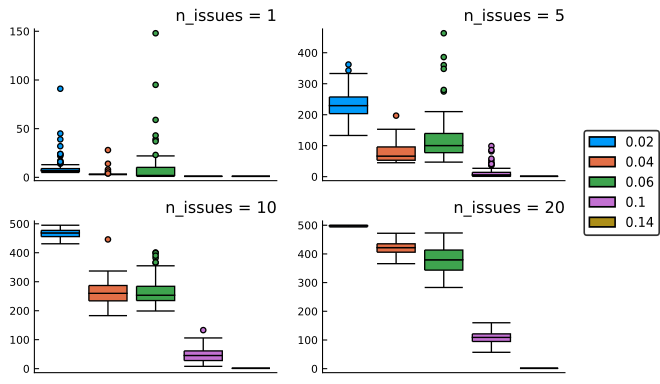
\includegraphics[scale=0.7]{ims/boxes4.png}
    \caption{Parametrização: \(\rho = p\_intran = 0.0, p = 0.9, N =500\)}
    \label{fig:box4}
  \end{figure}
  
  Como mostra a figura \ref{fig:box4} quanto maior o valor de \(\sigma\) menor a
  cobertura da configuração final. Contudo um resultado que aparenta ser
  contrário ao da análise anterior é que quanto maior o número de questões
  \textit{maior} a cobertura final, enquanto que a análise anterior demonstrou
  uma relação negativa entre número de questões e dispersão. Isso só é verdade,
  contudo, pelo fato dos parâmetros \(\rho\) e \(p\_intran\) serem nulos. Nesse
  caso aumentar o número de questões faz com que sejam necessárias mais
  interações entre os agentes para que eles se aproximem ideologicamente, já que
  pelo procedimento da simulação eles só atualizam uma opinião por vez. Isso faz
  com que aumentar o número de questões contribua para uma maior dispersão e
  cobertura de posicionamento ideológicos.

  
\begin{figure}[H]
    \centering
    \begin{subfigure}[b]{0.49\textwidth}
      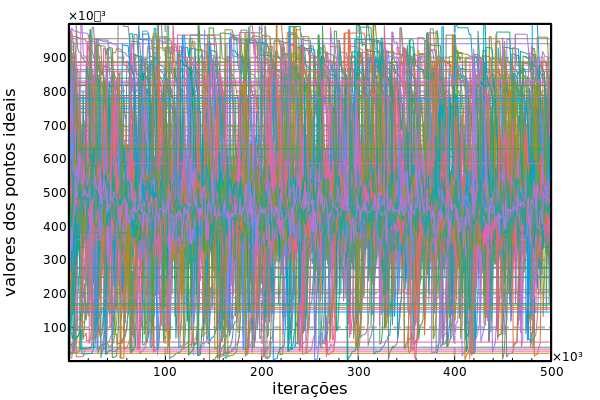
\includegraphics[width=\textwidth]{ims/n1-sigma01.png}
      \caption{\( n\_issues = 1,  \sigma = 0.1\) }
    \end{subfigure}
    \begin{subfigure}[b]{0.49\textwidth}
      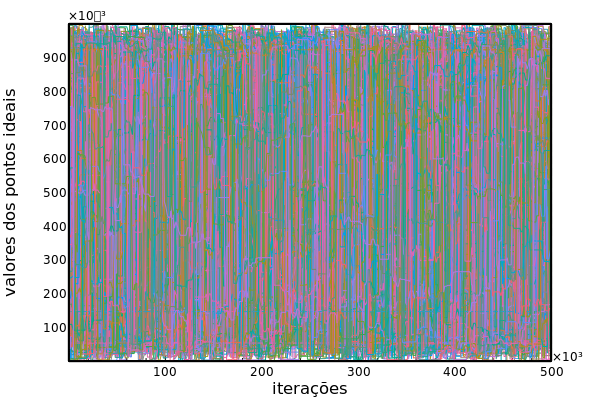
\includegraphics[width=\textwidth]{ims/n1-sigma002.png}
       \caption{\(n\_issues = 1, \sigma = 0.02\) }
     \end{subfigure}

     \begin{subfigure}[b]{0.49\textwidth}
       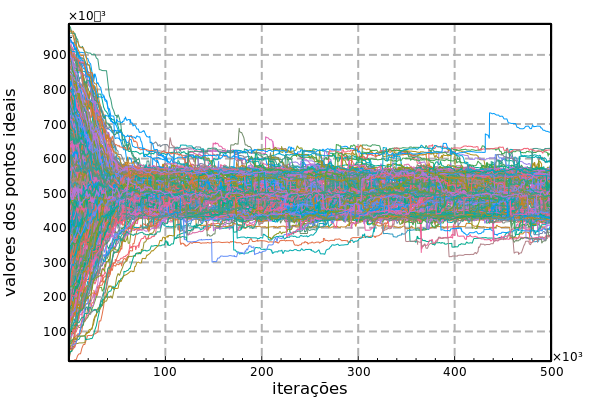
\includegraphics[width=\textwidth]{ims/n7-sigma01.png}
       \caption{\(n\_issues = 7, \sigma = 0.1\)}
     \end{subfigure}
     \begin{subfigure}[b]{0.49\textwidth}
       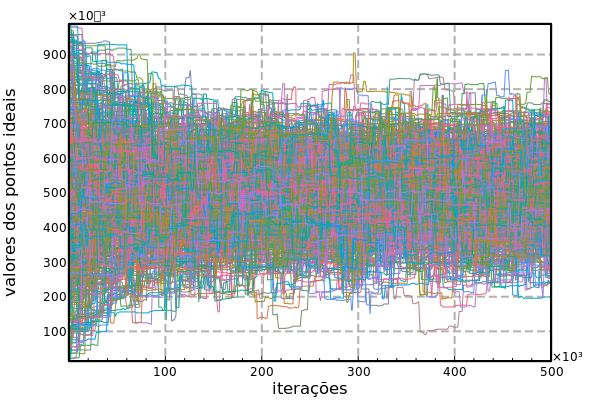
\includegraphics[width=\textwidth]{ims/n7-sigma002.png}
       \caption{\(n\_issues = 7, \sigma = 0.02\)}
     \end{subfigure}
      \caption{Evolução dos pontos ideais quando há ruído e agentes intransigentes.
        Parametrização: \(p\_intran = 0.15, \text{ } N = 500,  \text{ }   p =
        0.9,  \text{ }  \rho = 0.05\)}
      \label{fig:tseries4}
    \end{figure}
    
    Contudo, a partir do momento que a proporção de agentes intransigentes e o
    ruído são não-nulos o número de questões passa a ter o efeito contrário.
    Como demonstrado na figura \ref{fig:tseries4} quando \(n\_issues = 1\) o
    sistema passa a ter sua configuração facilmente controlada por aqueles
    parâmetros. Como só há uma única questão os agentes quando sofrem o efeito
    do ruído passeiam pelo espectro todo. Já quando interagem com agentes
    intransigentes tem seu ponto ideal atraído bem mais em direção a opinião
    deles, em contraposição ao caso em que seu ponto ideal é derivado de várias
    opiniões, pois mesmo que o agente mude, aleatoriamente ou sob o efeito da
    interação com um agente intransigentes, \textit{uma} de suas opiniões o
    ponto ideal é estabilizado pelo posicionamento dele em outras questões. O
    número de questões serve então para controlar o efeito dos agentes
    intransigentes e do ruído, e tornar mais robusto o efeito de concentração
    ditado por \(\sigma\), o parâmetro de maior impacto.




%%% Local  Variables:
%%% mode: latex
%%% TeX-master: "master"
%%% End:



\chapter*[Considerações Finais]{Considerações Finais}
\addcontentsline{toc}{chapter}{Considerações Finais}
  
    

\chapter*[Apêndice 1]{Apêndice 1 - Dos dados}
A primeira ressalva metodológica em relação aos dados é que não aplicamos os
pesos recomendados pelo \textit{European Social Survey}. Isso significa que,
dado o viés de seleção, as figuras representam o auto-posicionamento dos
respondentes, mas não da população \footnote{Escolhemos a Polônia para a Figura
  3, contudo, por ser o país com a menor variância do peso pós-estratificação.}.
Por não termos aplicado o peso que controla pelo tamanho das populações a Figura
4 não nos permite comparar o auto-posicionamento entre os países\footnote{Mesmo
  que tivéssemos aplicado o peso a comparação entre países usando um
  auto-posicionamento ideológico é complicado dado que a dimensão tem
  significados distintos em diferentes contextos \cite{laver2014measuring}. }.
Além de haver uma variação entre o tamanho das amostras, só representamos,
obviamente, respostas válidas, embora houvesse opção de responder ``Não sei''.



\begin{table}[h]
  \centering
\label{my-label}
\begin{tabular}{|l|r|r|}
\hline
\textbf{Países} & \textbf{N total} & \textbf{Fração  de Respostas  válidas} \\ \hline
Alemanha        & 2919             & 0.93                           \\ \hline
Bélgica         & 1899             & 0.86                           \\ \hline
Dinamarca       & 1506             & 0.93                           \\ \hline
Eslovênia       & 1519             & 0.79                           \\ \hline
Espanha         & 1729             & 0.81                           \\ \hline
Finlândia       & 2000             & 0.95                           \\ \hline
França          & 1503             & 0.94                           \\ \hline
Grécia          & 2566             & 0.77                           \\ \hline
Hungria         & 1685             & 0.83                           \\ \hline
Irlanda         & 2046             & 0.83                           \\ \hline
Israel          & 2499             & 0.92                           \\ \hline
Luxemburgo      & 1552             & 0.77                           \\ \hline
Noruega         & 2036             & 0.98                           \\ \hline
Países Baixos   & 2364             & 0.95                           \\ \hline
Polônia         & 2110             & 0.83                           \\ \hline
Portugal        & 1511             & 0.80                           \\ \hline
Reino Unido     & 2052             & 0.91                           \\ \hline
Suécia          & 1999             & 0.95                           \\ \hline
Suíça           & 2040             & 0.92                           \\ \hline
Áustria         & 2257             & 0.86                           \\ \hline
\end{tabular}
\caption{Número de Entrevistados (N) para 20 países do ESS 2002}
\end{table}


Outra ressalva é que as respostas são discretas (0-10) enquanto a teoria e nosso
modelo supõem pontos ideais num espaço contínuo. Uma solução é discretizar o
\textit{outcome} quando formos validá-lo. Outra é estimar as preferências dos
indivíduos por meio de suas respostas em outras perguntas do \textit{survey}
\footnote{Por meio, por exemplo, de técnicas de análise fatorial ou de componentes
  principais \cite{laver2014measuring}.}.

	
\postextual
	
% Referências bibliográficas
% ----------------------------------------------------------
\bibliography{master-bib.bib}
	
% ---------------------------------------------------------------------
% INDICE REMISSIVO
% ---------------------------------------------------------------------
\phantompart \printindex
% ---------------------------------------------------------------------
	
\end{document}
